%%%%%%%%%%%%%%%%%%%%%%%%%%%%%%%%%%%%%%%%%%%%%%%%%%%%
% Document type, global settings, and packages
%%%%%%%%%%%%%%%%%%%%%%%%%%%%%%%%%%%%%%%%%%%%%%%%%%%%


\documentclass[12pt]{report}   %12 point font for Times New Roman
\usepackage{graphicx}  %for images and plots
\usepackage[letterpaper, left=1.25in, right=1.25in, top=1in, bottom=1in]{geometry}
\usepackage{setspace}  %use this package to set linespacing as desired

\setcounter{tocdepth}{3}% Include \subsubsection in ToC
\setcounter{secnumdepth}{4}

\usepackage{times}  %set Times New Roman as the font
\usepackage{siunitx} % for Scientific notation

%%%%%%%%%%%%%%%%%%%%%%%%%%%%%%%%%%%%%%
% Setting Titles and Table of Contents
%%%%%%%%%%%%%%%%%%%%%%%%%%%%%%%%%%%%%%

\usepackage[explicit]{titlesec}  %title control and formatting
\usepackage[titles]{tocloft}  %table of contents control and formatting

%%%%%%%%%%%%%%%%%%%%%%%%%%%%%%%%%%%%%%
% Indent first Paragraphs
%%%%%%%%%%%%%%%%%%%%%%%%%%%%%%%%%%%%%%

\usepackage{indentfirst}

%%%%%%%%%%%%%%%%%%%%%%%%%%%%%%%%%%%
% Needed for Bibliography Compilation (could cause?)
%%%%%%%%%%%%%%%%%%%%%%%%%%%%%%%%%%%

\usepackage[backend=bibtex, sorting=none, bibstyle=ieee]{biblatex}  %reference manager

%%%%%%%%%%%%%%%%%%%%%%%%%%%%%%%%%%%
% More? Formatting (Checked)
%%%%%%%%%%%%%%%%%%%%%%%%%%%%%%%%%%%

\usepackage[bookmarks=true, hidelinks]{hyperref}
\usepackage[page]{appendix}  %for appendices
\usepackage{rotating}  %for rotated, landscape images
\usepackage[normalem]{ulem}  %for italicized text

%%%%%%%%%%%%%%%%%%%%%%%%%%%%%%%%%%%
% Math and Table Formatting (Checked)
%%%%%%%%%%%%%%%%%%%%%%%%%%%%%%%%%%%

\usepackage{amsmath} %facilitate writing math formulas

\usepackage{multirow}
\usepackage{mathtools}
\usepackage{array}
\usepackage{subcaption}
\usepackage{tabularx}
% to color the rows of table
\usepackage{color}
\usepackage{colortbl}

\usepackage{bm,amsmath,amssymb,color,subfigure}
\usepackage{breqn}  % <------ added here

%%%%%%%%%%%%%%%%%%%%%%%%%%%%%%%%%%%
% Vita (CV)
%%%%%%%%%%%%%%%%%%%%%%%%%%%%%%%%%%%

\usepackage{makeidx}
\usepackage{multirow}
\usepackage{multicol}
\usepackage[dvipsnames,svgnames,table]{xcolor}
\usepackage{graphicx}
\usepackage{epstopdf}
\usepackage{ulem}
%Already called
%\usepackage{hyperref}
\usepackage{amsmath}
\usepackage{amssymb}

%%%%%%%%%%%%%%%%%%%%%%%%%%%%%%%%%%%
% Bibliography
%%%%%%%%%%%%%%%%%%%%%%%%%%%%%%%%%%%

%Add your bibliography file here
\bibliography{references}

% prevent certain fields in references from printing in bibliography
\AtEveryBibitem{\clearfield{issn}}
\AtEveryBibitem{\clearlist{issn}}

\AtEveryBibitem{\clearfield{language}}
\AtEveryBibitem{\clearlist{language}}

\AtEveryBibitem{\clearfield{doi}}
\AtEveryBibitem{\clearlist{doi}}

\AtEveryBibitem{\clearfield{url}}
\AtEveryBibitem{\clearlist{url}}

\AtEveryBibitem{%
  \ifentrytype{online}
    {}
    {\clearfield{urlyear}\clearfield{urlmonth}\clearfield{urlday}}}

%%%%%%%%%%%%%%%%%%%%%%
% Nomenclatures
%%%%%%%%%%%%%%%%%%%%%%

\usepackage[utf8]{inputenc}
\usepackage{amssymb}
\usepackage{nomencl}
\makenomenclature


%% This will add the subgroups
%----------------------------------------------
\usepackage{etoolbox}
\renewcommand\nomgroup[1]{%
  \item[\bfseries
  \ifstrequal{#1}{A}{Analytical Expressions}{%
  \ifstrequal{#1}{B}{Number Sets}{%
  \ifstrequal{#1}{C}{Other Symbols}{}}}%
]}
%----------------------------------------------

%% This will add the units
%----------------------------------------------
\newcommand{\nomunit}[1]{%
\renewcommand{\nomentryend}{\hspace*{\fill}#1}}
%----------------------------------------------

%%%%%%%%%%%%%%%%%%%%%%%%%%%%%%%%%%%%%%%%%%%%%
% Used with Abbreviations & Glossary of Terms
%%%%%%%%%%%%%%%%%%%%%%%%%%%%%%%%%%%%%%%%%%%%%

\usepackage[utf8]{inputenc}
\usepackage[acronym]{glossaries}
\loadglsentries{glossary.tex}
\makeglossaries
%\renewcommand{\glossarypreamble}{\vspace*{-\baselineskip}}
\renewcommand*\glspostdescription{\dotfill}

%%%%%%%%%%%%%%%%%%%%%%%%%%%%%%%%%%%%%%%%%%%%%%%%%%%
% Cross referencing with the xr package in Overleaf
%%%%%%%%%%%%%%%%%%%%%%%%%%%%%%%%%%%%%%%%%%%%%%%%%%%

\usepackage{xr}

%%%%%%%%%%%%%%%%%%%%%%%%%%%%%%%%%%%%%%%%%%%%%%%%%%%%%%%%%%%%%%%%%%%%%%%%%%%%%%%%%%%%%%%%
%%%%%%%%%%%%%%%%%%%%%%%%%%%%%%%%%%%%%%%%%%%%%%%%%%%%%%%%%%%%%%%%%%%%%%%%%%%%%%%%%%%%%%%%
%%%%%%%%%%%%%%%%%%%%%%%%%%%%%%%%%%%%%%%%%%%%%%%%%%%%%%%%%%%%%%%%%%%%%%%%%%%%%%%%%%%%%%%%
% Start of Document
%%%%%%%%%%%%%%%%%%%%%%%%%%%%%%%%%%%%%%%%%%%%%%%%%%%%%%%%%%%%%%%%%%%%%%%%%%%%%%%%%%%%%%%%
%%%%%%%%%%%%%%%%%%%%%%%%%%%%%%%%%%%%%%%%%%%%%%%%%%%%%%%%%%%%%%%%%%%%%%%%%%%%%%%%%%%%%%%%
%%%%%%%%%%%%%%%%%%%%%%%%%%%%%%%%%%%%%%%%%%%%%%%%%%%%%%%%%%%%%%%%%%%%%%%%%%%%%%%%%%%%%%%%

\begin{document}
\doublespacing  %set line spacing

%%%%%%%%%%%%%%%%%%%%%%%%%%%%%%%%%%%%%
% Title Page
%%%%%%%%%%%%%%%%%%%%%%%%%%%%%%%%%%%%%

\currentpdfbookmark{Title Page}{01_titlePage}  %add PDF bookmark for this page
%% Define your thesis title, your name, your school, and your month and year of graduation here

\newcommand{\thesisTitle}{Investigating Accuracy of the  Reconfigurable Optical Computer (ROC) in Metatronics for Solving Partial Differential Equations}
\newcommand{\yourName}{Joseph Warren Crandall}
\newcommand{\yourSchool}{School of Engineering \& Applied Science}
\newcommand{\yourMonth}{May}
\newcommand{\yourDay}{19}
\newcommand{\yourYear}{2019}

%%%%%%%%%%%%%%%%%%%%%%%%%%%%%%%%%%%%%%%%%%%%%%%%%%%%%%%%%
% Do not edit these lines unless you wish to customize
% the template
%%%%%%%%%%%%%%%%%%%%%%%%%%%%%%%%%%%%%%%%%%%%%%%%%%%%%%%%%

\begin{titlepage}
\begin{center}

\begin{singlespacing}
\vspace*{1in}
\vspace{-\parskip}
\vspace{-\baselineskip}
\textbf{\thesisTitle}\\
\vspace{3\baselineskip}
by Joseph Warren Crandall\\
\vspace{3\baselineskip}
B.S. in Computer Science \& Physics, May 2017, The George Washington University\\
\vspace{3\baselineskip}
A Thesis submitted to\\
\vspace{1\baselineskip}
The Faculty of\\
The School of Engineering \& Applied Science\\
of the George Washington University\\
in partial fulfillment of the requirements\\
for the degree of Master of Science\\
\vspace{3\baselineskip}
\yourMonth{} \yourDay{}, \yourYear{}\\
\vspace{3\baselineskip}
Thesis directed by\\
\vspace{1\baselineskip}
Volker J. Sorger\\
Associate Professor of Electrical \& Computer Engineering
\vspace{\baselineskip}
\vfill
%Copyright \copyright{} \yourName{} \yourYear{}

\end{singlespacing}

\end{center}
\end{titlepage}




%%%%%%%%%%%%%%%%%%%%%%%%%%%%%%%%%%%%%
% Copyright Page
%%%%%%%%%%%%%%%%%%%%%%%%%%%%%%%%%%%%%

\pagenumbering{roman}
\setcounter{page}{2} % set the page number appropriately based on the number of intro pages
\currentpdfbookmark{Copyright}{02_copyright}  %add PDF bookmark for this page
%%%%%%%%%%%%%%%%%%%%%%%%%%%%%%%%%%%%%%%%%%%%%%%%%%%%%%%%%
% Do not edit these lines unless you wish to customize
% the template
%%%%%%%%%%%%%%%%%%%%%%%%%%%%%%%%%%%%%%%%%%%%%%%%%%%%%%%%%
\clearpage

\begin{singlespacing}
\begin{center}
\vspace*{\fill}
\copyright{} Copyright \yourYear{} \yourName{}\\
All rights reserved
\vspace*{\fill}
\end{center}
\end{singlespacing}

\clearpage






%%%%%%%%%%%%%%%%%%%%%%%%%%%%%%%%%%%%%
% Dedication
%%%%%%%%%%%%%%%%%%%%%%%%%%%%%%%%%%%%%

\phantomsection
\addcontentsline{toc}{chapter}{Dedication}
%\currentpdfbookmark{Dedication_new}{03_dedication}  %add PDF bookmark for this page
\clearpage
\begin{centering}
\textbf{Dedication}\\
\vspace{\baselineskip}
\end{centering}

%Insert your dedication text here
This work is dedicated to my family and friends who motivate and support me. Thank you all.

\clearpage
%\pagenumbering{gobble}  %remove page number on summary page

%%%%%%%%%%%%%%%%%%%%%%%%%%%%%%%%%%%%%
% Acknowledgments
%%%%%%%%%%%%%%%%%%%%%%%%%%%%%%%%%%%%%

\phantomsection
\addcontentsline{toc}{chapter}{Acknowledgments}
\clearpage
\begin{centering}
\textbf{Acknowledgments}\\
\vspace{\baselineskip}
\end{centering}

%Insert your Acknowledgement text here
The research environment at GW has provided me with time, equipment, and colleagues to learn from and collaborate with, some of which I would like to thank explicitly. Engin Kayraklioglu has been instrumental in the development of the first iteration of the ROC software stack which includes SPICE models, usage of the Lumerical API, and is now starting to focus on error correction and will eventually involve ROC drivers. I hope to keep collaborating with you on this GitHub repository. Shuai Sun has been my desk mate ever since I started working in the OPEN Lab. He has led the fabrication of photonic ROC as well as being one of the first people in the Lab to learn the Lumerical simulation tool set. I have asked Shuai many questions and he has answered even more. Even since the arrival of our Postdoc Mario Miscuglio, my research has been accelerated. Mario's depth and breath of photonic and metatronic knowledge and modeling skill has motivated me to improve me own. PI Tarek El-Ghazawi has provided extensive edits throughout the thesis process and I greatly appreciate his input. Finally I would like to thank my PI Volker Sorger for both his edits during the thesis writing process and for pushing this team aggressively and helping to put us on the map. Thank you all.

\clearpage
%\pagenumbering{gobble}  %remove page number on summary page


%%%%%%%%%%%%%%%%%%%%%%%%%%%%%%%%%%%%%
% Abstract
%%%%%%%%%%%%%%%%%%%%%%%%%%%%%%%%%%%%%

\phantomsection
\addcontentsline{toc}{chapter}{Abstract of Thesis}
\begin{center}
\textbf{Abstract of Thesis}
\begin{singlespace}
\textbf{Investigating Accuracy of the  Reconfigurable Optical Computer (ROC) in Metatronics for Solving Partial Differential Equations}
\end{singlespace}
\end{center}

\par Nanoscale area metatronic analog circuitry utilizes relative permittivity between material interfaces to confine and direct electric displacement field and electric displacement current density operating at $f = \SI{193}{T\hertz}$. This is interesting because we have shown that we can map an analog finite difference algorithm into metatronics, while avoiding the \acrfull{pde} decreasing accuracy at increasing node density issue encountered by microscale area photonic analog circuitry also operating at $f = \SI{193}{T\hertz}$ 

\par The microscale area electronic analog circuitry, operating at $f \approx \SI{300}{G\hertz}$, and the nanoscale area metatronic circuitry both exhibit \acrfull{pde} solution increasing accuracy at increasing node density, in the same fashion to a software driven digital hardware based finite difference algorithm \acrshort{pde} solution approaching the accuracy of analytically derived pde solution through increased node density.

\par With the proper allocation of hardware source and sample location for the metatronic and electronic circuitry we have shown that both analog hardwares can operate in constant time $0(1)$, and thus merit integration into larger software based parallel multi grid methods. However, the larger metatronic operating frequency increases its Shannon–Hartley theorem limited repetition rate (clock speed) into the Terahertz, while the smaller electronic operating frequency relegates its Shannon–Hartley theorem limited repetition rate (clock speed) to the Gigahertz.

\par Through the use of resistors, capacitors, and inductors the electronic circuit can be reconfigured to solve Laplace, Poisson, diffusion, and wave partial differential equations. In principal the metatronic circuit can bias its epsilon near zero material to induce changes in its relative permittivity inducing metatronic capacitance and inductance. Although this has not been shown in simulation at this point. Metatronic resistance occurs when the imaginary components of the epsilon near zeros material is not equal to zero.

\par It is difficult to understand all of the constraints one must account for in hardware design if one does not fully understand the final application the hardware solves. Any \acrshort{pde} solution method that employs a mesh or grid, and ultimately a finite difference, in the process of generating a solution suffers from discretization error. The only method that does not are analytically derived solutions, which is why it is important to understand what makes analytical methods challenging and not widely used, because in theory, the \acrshort{pde} solutions they produce will be the most accurate.

\par The mapping of a digital finite difference algorithm to an analog circuit requires the operational frequency and corresponding wavelengths size to exceed the diameter of the analog grid. This relationship determines the behavior of the electronic lumped, photonic distributed, and metatronic lumped grid based algorithms accuracy when solving \acrshort{pde}s. A lumped circuit node directs current, or displacement current density based on the direction and magnitude that the node's neighborhood is directing their current or displacement current density. In the case of a lumped circuit the neighborhood of nodes is the entire circuit. In a distributed circuit each nodes neighborhood is defined as all the nodes within one wavelength of operation. If the distance between two adjacent nodes is greater than one wavelength of operation, as is the case in the current fabricated photonic circuit, then all of the nodes are isolated. An isolated node does not feel the effects of a neighborhood because it has none, and instead must determine a new way to direct its optical intensity. The current practice is to engineer the geometry of the node to direct an equal amount of incoming optical intensity into all of the outgoing waveguides. This equal splitting is fixed in passive silicon.

\Par The effects on \acrshort{pde} accuracy of lumped neighborhood based variable splitting versus distributed isolated node fixed splitting begin to reveal themselves as the number of nodes in the circuit increases. Changes in grid size, density, or both point to a trend of increasing accuracy for the lumped element circuits and decreasing accuracy for the isolated node circuits when compared to analytical continuous and digital numerical discrete pde solutions.

\par This Thesis' findings encompassing the combined advantages of increasing accuracy, preserved reconfigurability, increased repetition rate, and decreased footprint for metatronic circuits solving \acrlong{pde}s paves the wave for experimental fabricated demonstrations to validate this theoretical work.

\clearpage
%\pagenumbering{gobble}  %remove page number on summary page

%%%%%%%%%%%%%%%%%%%%%%%%%%%%%%%%%%%%%
% Table of Contents
%%%%%%%%%%%%%%%%%%%%%%%%%%%%%%%%%%%%%

% Format for Table of Contents
\renewcommand{\cftchapdotsep}{\cftdotsep}  %add dot separators
\renewcommand{\cftchapfont}{\bfseries}  %set title font weight
\renewcommand{\cftchappagefont}{}  %set page number font weight
\renewcommand{\cftchappresnum}{Chapter }
\renewcommand{\cftchapaftersnum}{:}
\renewcommand{\cftchapnumwidth}{5em}

\renewcommand{\cftchapafterpnum}{\vskip\baselineskip} %set correct spacing for entries in single space environment
\renewcommand{\cftsecafterpnum}{\vskip\baselineskip}  %set correct spacing for entries in single space environment
\renewcommand{\cftsubsecafterpnum}{\vskip\baselineskip} %set correct spacing for entries in single space environment
\renewcommand{\cftsubsubsecafterpnum}{\vskip\baselineskip} %set correct spacing for entries in single space environment

%format title font size and position (this also applies to list of figures and list of tables)
\titleformat{\chapter}[hang]{\normalfont\bfseries\filcenter}{\chaptertitlename\ \thechapter}{0pt}{#1}
\titlespacing*{\chapter}{0pt}{-16pt}{12pt}	%controls vertical margins on title
\renewcommand\contentsname{Table of Contents}
\currentpdfbookmark{Table of Contents}{TOC}
\begin{singlespace}
\tableofcontents
\end{singlespace}

\clearpage

%%%%%%%%%%%%%%%%%%%%%%%%%%%%%%%%%%%%%
% List of figures and tables
%%%%%%%%%%%%%%%%%%%%%%%%%%%%%%%%%%%%%

\phantomsection
\addcontentsline{toc}{chapter}{List of Figures}
\begin{singlespace}
\setlength\cftbeforefigskip{\baselineskip}  %manually set spacing between entries
%\currentpdfbookmark{List of Figures_new}{LOF}  %add PDF bookmark for this page
\listoffigures
\end{singlespace}

\clearpage

%\phantomsection
%\addcontentsline{toc}{chapter}{List of Tables}
%\begin{singlespace}
%	\setlength\cftbeforetabskip{\baselineskip}  %manually set spacing between entries
	%\currentpdfbookmark{List of Tables_new}{LOT}  %add PDF bookmark for this page
%	\listoftables
%\end{singlespace}

%\clearpage

%%%%%%%%%%%%%%%%%%%%%%%%%%%%%%%%%%%%%
% Nomenclature
%%%%%%%%%%%%%%%%%%%%%%%%%%%%%%%%%%%%%

%\phantomsection
%\addcontentsline{toc}{chapter}{Nomenclature}
%\currentpdfbookmark{Nomenclature_new}{N}  %add PDF bookmark for this page
%\printnomenclature
%\clearpage

%%%%%%%%%%%%%%%%%%%%%%%%%%%%%%%%%%%%%%%%%%%
% List of Abbreviations 
%%%%%%%%%%%%%%%%%%%%%%%%%%%%%%%%%%%%%%%%%%%

\phantomsection
\addcontentsline{toc}{chapter}{List of Abbreviations}
%\currentpdfbookmark{List of Abbreviations_new}{LOA}  %add PDF bookmark for this page
\printglossary[type=\acronymtype,title=List of Abbreviations]
\clearpage

%%%%%%%%%%%%%%%%%%%%%%%%%%%%%%%%%%%%%%%%%%%
% Glossary of Terms
%%%%%%%%%%%%%%%%%%%%%%%%%%%%%%%%%%%%%%%%%%%

\phantomsection
\addcontentsline{toc}{chapter}{Glossary of Terms}
%\currentpdfbookmark{Glossary of Terms_new}{GOT}  %add PDF bookmark for this page
\printglossary[title=Glossary of Terms]
\clearpage

%%%%%%%%%%%%%%%%%%%%%%%%%%%%
%
% Chapters
%
%%%%%%%%%%%%%%%%%%%%%%%%%%%%

%%%%%%%%%%%%%%%%%%%%%%%%%%%%
% formatting
%%%%%%%%%%%%%%%%%%%%%%%%%%%%

% resume page numbering for rest of document
\clearpage
\pagenumbering{arabic}
\setcounter{page}{1} % set the page number appropriately

% Adjust chapter title formatting
\titleformat{\chapter}
[hang] %
{\normalfont\bfseries\filcenter} %spacing between titles
{\chaptertitlename\ \thechapter\ -}
{2pt}
{{#1}}  %spacing between titles

\titlespacing*{\chapter}{0pt}{0pt}{0pt}	%controls vertical margins on title
  
% Adjust section title formatting
\titleformat{\section}{\normalfont\bfseries}{\thesection}{1em}{#1}

% Adjust subsection title formatting
\titleformat{\subsection}{\normalfont}{\uline{\thesubsection}}{0em}{\uline{\hspace{1em}#1}}

% Adjust subsubsection title formatting
\titleformat{\subsubsection}{\normalfont}{\uline{\thesubsubsection}}{0em}{\uline{\hspace{1em}#1}}

%%%%%%%%%%%%%%%%
% Chapter 1 
%%%%%%%%%%%%%%%%

\chapter{Introduction}

\section{What is ROC}\label{whatROC}
\acrfull{roc} is research project undertaken by a collaboration between the OPEN Lab Team under the leadership of PI Volker Sorger and the HPCL Team under the leadership of PI Tarek El Ghazawi both based at the George Washington University through the funding of an NSF RAISE Grant working to understanding the physics of, develop software for, and fabricate an analog co-processor implemented in Silicon Photonics, and Optical Metatronics, with the goal of calculating approximate solutions to 4 classes of partial differential equations comprised of Laplace, Poisson, Diffusion, and Wave. The approximate accuracy of these solutions, the time required to attain them, the energy utilized in the computation, and the physical dimension of the fabricated chip are compared against analytically derived, and numerically computed solutions, as well against a previously researched electronic analog co-processor.

\par This research is part of a larger trend punctuated by the termination of the \gls{International Technology Roadmap for Semiconductors} (\acrshort{itrs}) 2.0 report with its final 2015 publication \cite{itrs2.0_2015}. The report published for decades comprised an amalgamation of the opinions of worlds leading semiconductor researchers and industry professionals and is arguably most known for setting expectations for semiconductor \gls{technology node} scaling. However due to the challenges posed by the limits of \gls{Moore's law}, the end of \gls{Dennard scaling}, the slowing of \gls{Koomey's law}, and the limits of \gls{Amdahl's Law}. 

\par The \gls{Institute of Electrical and Electronics Engineers} (\acrshort{IEEE}) has pivoted and released the \gls{International Roadmap For Devices And Systems} (\acrshort{irds}) 2017 edition \cite{irds_2017}. In the report \acrshort{irds} acknowledges that 2D scaling will reach fundamental limits beyond 2020 and as a solution they introduce three distinct eras of scaling, Geometrical (1975-2002), Equivalent (2003 $\sim$ 2024), and 3D Power (2025 $\sim$ 2040) with Equivalent Scaling (2003 $\sim$ 2024) being defined by the "reduction of only horizontal dimension in conjunction with introduction of new materials and new physical effects". With "new vertical structures replacing planar transistors". Our research embraces this paradigm shift and falls within the scope of new materials and new physical effects. As of 2018 companies such as Xilinx have started to design processors with CPU, GPU, and FPGA architectures integrated \cite{vissers2019versal}, with the new question being which architecture is best for which task. The PDE co-processing capabilities of ROC fall within this trend.


\section{Papers, Patents, and Challenges}
\par The concept of an analog electronic mesh based computer applied to approximately solve partial differential equations was initially researched by G. Liebmann and colleagues in the 1950's \cite{G.Liebmann_1950, liebmann1954resistance}. In 2000, a programmable \gls{Very Large Scale Integration} (\acrshort{vlsi}) chip for analog solutions to \acrshort{pde}s was patented \cite{ramirez2000digitally} that can be implemented using discrete components or as an \gls{application-specific integrated circuit} (\acrshort{asic}), hosted by a digital computer. In 2015 members of the \acrfull{hpcl} and \acrfull{open} lab and the filed a patent for an optical implementation of a \acrshort{pde} solving circuit implementation of \acrfull{roc} \cite{patent_20170161417}.

\par Due to the focused time I have spent working on the 4 year (2017-2021) \acrfull{nsf} \acrfull{raise} funded \acrshort{roc} project I have been able to uncover the underlying challenges I have been working to address as well as the ones that I have avoided in my goal of understanding accuracy.The ROC project is a product of larger research trend, partially encompassed by what I believe are two grand challenges. 

\par The first being that CMOS technology surpassed analog alternatives in the 1970s because of its versatility and successful scaling, but decreasing CMOS 2D length scaling is ending during the 2020s, which is creating room for many alternative technologies to be proposed. This research space and funding created by the first challenge has allowed teams to think fundamentally about how different algorithms perform computation. After working on the ROC project, I have come to the conclusion that I am sure many other researchers before me have concerning competitiveness encompassed in the second grand challenge. 

\par Algorithms built into hardware must improve their computational time complexity compared to pure software-based implementations to make up for a loss of versatility, but how much versatility must the hardware provide for the effort to be worthwhile? I realize that algorithms built into hardware can have similar computational time complexity but improved energy consumption compared to pure software, but since I am focusing on accuracy as a metric of performance, I ahve not rigorously explore improvements in energy consumption as a metric of performance.


\section{Deliverables}
\par My thesis is composed of three chapters, Context & Motivation, Mathematics & Physics Underlying the Computation Model, and Future Work. The Context & Motivation chapter discusses the intellectual discoveries the word builds on as well as challenges I am working to understand and address. The deliverable discussed correspond to my contributions to the yearly NSF specified project requirements and the structure of the written thesis. The partial differential equation solution methods cover the different ways one can go about solving a PDE and their limitations. The reconfigurable optical computer operation gives an overview of the physical photonic and metatronic analog coprocessors used to solve the PDEs, and accuracy covers the metric I use to evaluate the performance of the computer.

\par The second chapter, the Mathematics & Physics Underlying the Computational Model contains the meat of my investigation. In a top down approach, I first ask the question where do the computational complexity gains originate from in an analog approach compared to a numerical discrete one? I then analytically derive a solution to a partial differential equation in order to understand where the difficulty in analytical approaches arises from and why an algorithmic analytical approach to pde solutions is challenging. Then I show the standard numerical approach to a pde solution, followed by the original electrical analog approach and then the novel Photonic analog and Metatronic analog approaches. In the future work chapter I touch on what is expected by the NSF for the team to accomplish in the remaining two years as well as further Metatronic work that I am hoping to complete.

\subsection{Year 1 from October 2017 to September 2018}
\par During the first year of the NSF Project I created a branch of the "roc_grid_simulation" GitHub repository, initially developed by Engin Kayraklioglu, named boundaryConditions utilizing Python to generate spice based simulations of the electrical grid used by Lieberman to calculate their accuracy compared to an analytical solution to a Laplace PDE solution that I had derived. In order to better understand Liebmann’s finite difference mapping technique I re derived his work which helped me understand the importance of a node and its neighborhood in terms of this relationships effect on accuracy and how it is altered with the physics of Photonics and Metatronics.

\subsection{Year 2 from October 2018 to September 2019}
\par During the second year I created COMSOL Models of the Metatronic ROC in order to study the effects of network size and density on their role in accuracy, leading to an understanding of the importance of \gls{displacement current density} confinement. In my desire to showcase the possible computational advantages of ROC, I estimated computational time complexities values for the future processor in comparison to an electrical analog and how it could be utilized within a and discrete parallelized implementation.


\section{Partial Differential Equation Solution Methods}
\par Many computational problems in science and engineering are modeled via solving partial differential equations (PDEs) and are used to model physical phenomena such as fluid dynamics \cite{Isom_H._2008}, electricity \cite{M.Sadiku_1990}, magnetism \cite{H.Berestycki_2002}, mechanics \cite{A.Selvadurai_2000}, optics \cite{C.Tang_2013}, and heat flow \cite{rocca2015entropic}. Some of these problems can not be solved for an \gls{Analytic expression} and must rely on \gls{Numerical analysis} to generate a final answer. Numerically derived solutions are commonly solved by first discretizing them into finite difference equations or finite elements through the use of the \gls{finite difference method}. Iterative methods such as \gls{Conjugate gradient method} or the adaptive \gls{Multigrid method} are also often adopted in order to solve these equations \cite{richter2015memristive}. Due to the large number of iterations in the recursive process required to attain more accurate solutions.

\par Due to the computational energy and time expense required to solve these equations techniques have been invented to simplify their calculation, such as transforming the \acrshort{pde}s into ordinary differential equations \gls{ordinary differential equation} (\acrshort{ode}s) and much attention has been paid to creating efficient implementations of \acrshort{pde} solvers aimed at reducing the number of iterations \cite{J.Zhu_1994, L.Pinuel_1998}. A \acrshort{pde} solution of heat flow over a homogeneous surface computed numerically requires the decomposition of the surface into an array of subsurfaces through the finite difference method, known as a computational mesh.  Subsurfaces with smaller areas yield higher-precision results, but require more computations to arrive at a solution. As PDEs form the basis for many applications in scientific computing, efficiencies gained in this domain would be of great benefit to the scientific community \cite{J.Dongarra_2017}.

\par The analog alternative to this digitally implemented numerical method traditionally utilized analogue circuits comprised of Resistor(R), Inductor(L), and Capacitor (C) elements that bypass the iterative recursive process by generating a mesh based solution in a single execution, equivalent to a computational complexity \gls{Big O notation} of 1 or $n$ (linear) depending on the speed of execution, once boundary conditions for the problem are set within the mesh, with the accuracy of the solution being determined by combination of the density of the mesh utilized and the area of the problem being solved for. This electrical analog finite difference architecture utilizes summation of current for computation and  was originally developed to provide efficient computation of heat transfer \cite{G.Liebmann_1950} and oscillatory flow problems in aeronautical engineering \cite{P.Palmer_1959}, and has been shown to reduce the time to solution through its elimination of the iterative processing steps which retard numerical methods.

Solving \acrshort{pde}s using Electrical Analogues requires an array of circuit elements suitably connected in order to yield electrical analogue of a PDE. A two-dimensional resistor array can generate an analog solution to a Laplace equation,

\begin{equation}\label{Laplace}
\nabla^2 \varphi = 0
\end{equation}
\nomenclature[A]{$\nabla^2$}{Laplace operator}
\nomenclature[A]{$\varphi$}{A twice-differentiable real-valued function}

while sampling current at nodes, we expand the class of PDEs to non zero solution Poisson Equations,

\begin{equation}\label{Poisson}
\nabla^2 \varphi = ki
\end{equation}
\nomenclature[A]{$ki$}{Real or complex-valued function on a manifold}

with the addition of capacitors at at nodes, we account for time dependence and expand the class of \acrshort{pde}s to Diffusion Equations,

\begin{equation}\label{Diffusion}
\nabla^2 \varphi = k \frac{\partial \varphi}{\partial t }
\end{equation}

and by substituting capacitors for resistors and keeping capacitors at nodes, we expand the class of \acrshort{pde}s to Wave Equations,

\begin{equation}\label{Wave}
\nabla^2 \varphi = k \frac{\partial^2 \varphi}{\partial t^2}
\end{equation}

These classes of PDEs that can be accelerated by an electronic analog mesh based co-processor each solve problems in a specific application-space and cater to a wide spectrum of the standard simulation applications in science and engineering. 

\begin{figure}[ht]
    \centering\fbox{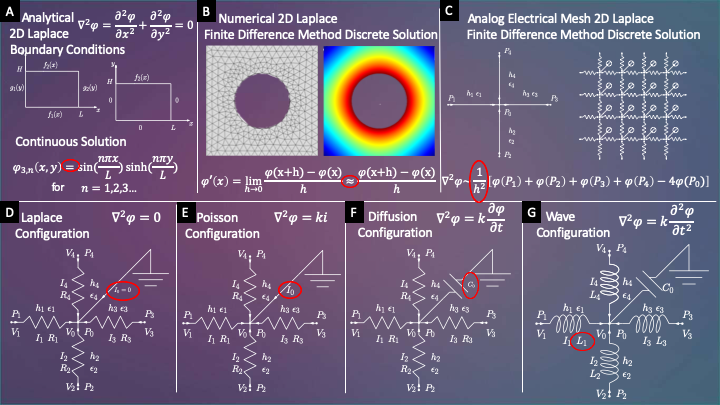
\includegraphics[height=3in, width=5.5in]{figures/figures1/01_analytical_numerical_analog.png}}
    \caption{The top row of this figure illustrates the traditional options available for solving a PDE through \textbf{(A)} analytical, \textbf{(B)} numerical, and \textbf{(C)} analog electrical PDE solving paradigms, while the bottom row illustrates the reconfigurations of an analog electrical discrete solution for different classes of \acrfull{pde}s including \textbf{(D)} Laplace, \textbf{(E)} Poisson, \textbf{(F)} diffusion, and \textbf{(G)} wave equation.}
    \label{fig:01_analytical_numerical_analog}
\end{figure}

Due to complexities surrounding the effective integration of a static analog mesh computer in a \acrfull{vlsi} architecture, the resistance network analogue has remained in the academic domain \cite{J.Ramirez-Angulo_2000}. This shortcoming was improved upon by Ramirez-Angulo and DeYong \cite{J.Ramirez-Angulo_2000} with a VLSI-friendly implementation of an analog mesh computer using Complementary Metal Oxide Semiconductor (CMOS) transistors operated in the subthreshold regime.  However, modern digital VLSI designs prefer the use of minimum-size devices, which is at odds with subthreshold CMOS designs, which require larger devices to ensure proper matching \cite{A.Hastings_2005}.  

\par Recent programs advocating for new and innovative computer architectures \cite{darpa2017}, and the recent introduction of innovative, programmable VLSI devices, such as the nanophotonic modulator \cite{V.Sorger_2012}, have created opportunities for innovative architectures that can take advantage of these new devices \cite{A.Mehrabia_2018,S.Sun_2018}. Conceptual metastructure based analog computing models are starting to be developed by leaders in the field including Nader Engheta \cite{Mohammadi_Estakhri1333}.  In the telecommunications space, Photonic ROC can potentially be used to efficiently model \gls{multiple-input and multiple-output} (\acrshort{mimo}) systems that make substantial use of \acrshort{pde}s \cite{tsoulos2006mimo}. The recent push for \gls{post-Moore} computer architectures \cite{darpa2017}, has introduced a wide variety of application-specific accelerators \cite{hu2016dot,bojnordi2016memristive,J.George_2017}.  Generally, these accelerators are designed to improve the performance of computationally-intensive algorithms by limiting unnecessary calculations or data movements. To maximize an application-specific computer's utility, it must be capable of accelerating widely used algorithms. The progression to an analog electrical \acrshort{pde} solution accelerator is shown in Figure \ref{fig:01_analytical_numerical_analog}.


\section{ROC Fundamentals}
\subsection {ROC}

\acrfull{roc} is a reconfigurable optical wavelength \\ \gls{co-processor}, implemented in two distinct physical technologies, capable of approximately solving \acrshort{pde}s through the \gls{finite difference method}, constructed in a physical analog mesh but differing from the electrical implementation introduced in Figure \ref{fig:01_analytical_numerical_analog} by performing summation of electrical \gls{displacement current} desnity for \gls{Metatronic} \acrshort{roc} and summation of \gls{optical intensity} in \gls{Photonic} \acrshort{roc}. 

\par Increases in the \gls{RC time constant} as a 2D electric mesh scales its number of nodes quadratically increases signal delay across the diameter of the mesh. If this signal delay exceeds the clock speed of the processor the computational time complexity of the analog electrical mesh degrades from $O(1)$ to $O(n)$ where $n$ is the number of nodes along a single side of a square mesh.

\par Different electrical meshes, as shown in Figure \ref{fig:01_analytical_numerical_analog}, must be fabricated for different configurations of \acrshort{pde}s, therefore making an electronic analog static co-processor non reconfigurable.

\par Static photonic \acrshort{roc} utilizes changes in optical intensity due to optical loss to solve Laplace and Poisson \acrshort{pde}s. \gls{Metatronic} \acrshort{roc} confines electric displacement current density $J_D = \frac{\partial D}{\partial t}$ in epsilon vary large (EVL) materials surrounded by epsilon near zero (ENZ) materials and directs $J_D$ through nano-inductors, nano-capacitors, and nano-resistors.

\par The ability to change the accuracy of the \acrshort{pde} solution through the ratio of the density of the mesh versus the area of the \acrshort{pde} being solved for makes the \acrshort{roc} co-processor concept appropriate for future Energy-Quality (EQ) scalable systems, advocated for by  green computing initiatives, which require the ability to explicitly trade off energy and quality at different levels of abstraction \cite{M.Alioto_2017}.

\begin{figure}[ht]
\centering\fbox{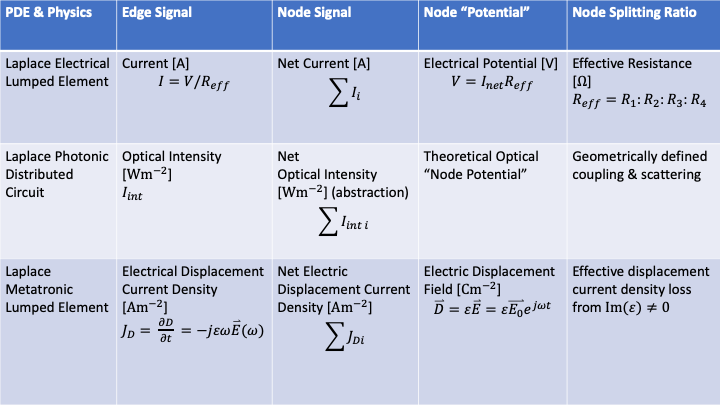
\includegraphics[height=3.5in, width=6in]{figures/figures1/02b_physics_table.png}}
\caption{The Laplace \acrshort{pde} dependent physical units and equations for grid components in the electronic mesh, photonic \acrshort{roc}, and metatronic \acrshort{roc} are shown. The electrical and metatronic circuits operate as lumped elements and the photonic circuit operates as a distributed circuit. The equation units of metatronic \acrshort{roc} electric displacement current density are as follows: $\tilde{\varepsilon}$ material permittivity [\si{\farad \meter^{-1}}], $\omega = 2\pi f$ Angular Frequency [\si{\hertz}], $E(\omega)$ electrical field [\si{\volt \meter^{-1}}] or [\SI{}{\newton \coulomb^{-1}}]. It is also important to distinguish between which photonic quantity's are measurable. We measure optical intensity through the use of a Y branch and a grating along each edge at the output of each optical node.}
\label{fig:01_02b_physics_table}
\end{figure}


\subsection{Photonic}

\par Passive photonic ROC utilizes pure etched silicon waveguides and ring resonators combined with an central splitting element combined to form a photonic device that directs light evenly from the input port to the 3 output ports with a 33.3\% 33.3\% 33.4\%  splitting. Photoinc ROC is fabricated within the GW clean room and is at a length scale greater than the wavelength of light, $\lambda = \SI{1550}{n\meter}$ being using. The distance form node to node is $h = \SI{60}{u\meter}$. This size differential results in Photoinc ROC operating in accordance to the \gls{distributed element model} shown in Figure \ref{fig:01_02_electrical_photoinc_metatronic}. 

\par Unfortunately there is a weak mapping of the electrical mesh to the photonic Mesh. This is because we must attempt to replicate electrical resistance with optical loss which is not equivalent. We also do not have a photonic equivalent to electrical capacitance or electrical inductance. However due to the relative ease of manufacturing a photonic mesh compared to a metatronic mesh we have invested energy and time into the photonic implementation of ROC as a way to demonstrate an initial fabrication. However the combination of equal splitting along with the distributed element model means that as we scale ROC for larger numbers of nodes the overall accuracy of the PDE solution decreases which is the opposite of what is desired for a analog finite difference algorithm as it is scaled up as noted in Figure \ref{fig:1_03a_elec_accuracy}.

\begin{figure}[ht]
\centering\fbox{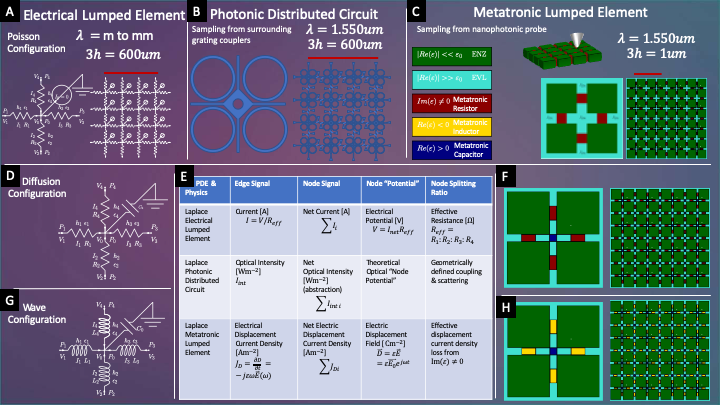
\includegraphics[height=3.5in, width=6in]{figures/figures1/02_electrical_photonic_metatronic.png}}
\caption{ The top row of this figure illustrates the different analog grid based \acrshort{pde} solving technologies including \textbf{(A)} the original electrical analog, \textbf{(B)} the silicon photonics implementation, and \textbf{(C)} the Metatronic Implementation. The columns represent the different configurations of the grid, that give the “reconfigurable” optical computer its name, allowing for Poisson, diffusion, and wave configurations. 
As you probably have noticed, there is no photonic schematic showing an equivalence to \textbf{(D)} electrical capacitance, or \textbf{(G)} electrical inductance, but there is \textbf{(F)} metatronic capacitance and \textbf{(H)} metatronic inductance. Table \textbf{(E)} shows the physical effects utilized in the technologies and is shown in larger form in Figure \ref{fig:01_02b_physics_table}. In the language of graph theory, a node is a grid point within the mesh, and an edge is a connection between grid points.}
\label{fig:01_02_electrical_photoinc_metatronic}
\end{figure}

\subsection{Metatronic}

\par In microelectronics and combination of an electrical current and electrical potential through lumped elements including resistors, inductors, and capacitors has led to successful modularization of circuit design through the radio frequency and microwave domains. As we have seen in the photonic case, operating in the optical domain while still benefiting from a lumped circuit paradigm is not trivial. As Nadar Engatar stated in his 2007 Science paper \cite{N.Engheta_2007} there are two primary challenges to overcome. In lower frequency domains, designs involve elements that are much smaller than the wavelength of operation, fabrication techniques can be used to construct sub wavelength dimensions at optical wavelengths. Secondly the response of metals at IR and optical frequencies cannot be scaled directly from RF to optics.

\par The ideal metamaterial-based implementation of ROC with epsilon near zero set equal to zero as well as physically possible epsilon near zero values are simulated in the \gls{COMPSOL Multiphysics} based metatronic solution. of \acrshort{roc}.  Upper bounds are placed on the accuracy by $\lambda/L$, where $L$ is the feature size of the network components, due to the physical nature of light, and $\lambda$ is the wavelength.  

\par Metatronics enable the ideal ROC implementation, in terms of size and accuracy. However, the complexities of an effective integration of a high speed programmable and concurrently energy efficient static-like analog mesh significantly reduced the advancement of this technology.  Here, we demonstrate the implementation of a nano-optic co-processor able to solve partial differential equation based on a metatronic nanocircuit board. 

\par Thanks to a unprecedented control of the \acrfull{enz} and material losses over \gls{Indium tin oxide} (\acrshort{ito}), we use different deposition conditions, in order to tune the \acrshort{enz} position, which potentially leads to a top-down monolithically integrated circuit \cite{gui2018impact}. The elements of the circuit could be then be electrostatically tuned \cite{amin20180, ma2015indium, alu2018metasurfaces, tahersima2017testbeds} and reprogrammable aiming to solve a variety of PDEs including Poisson, diffusion, and wave. 

\par A discussion on losses and physical limitation, induced by the losses of the ITO at ENZ condition is provided. The solution accuracy and its scaling functions are estimated for to finite difference approaches, and compared to other mesh solutions. The implementation of an all optical read-out paradigm is discussed based on a Nanophotonic \gls{probe card} that detects the local near field of the scattered field and provides information of a dielectric displacement, at given points of the nano-optics circuit, thus allowing to extrapolate the results of the computation. 


\section{Accuracy}
\begin{figure}[ht]
\centering\fbox{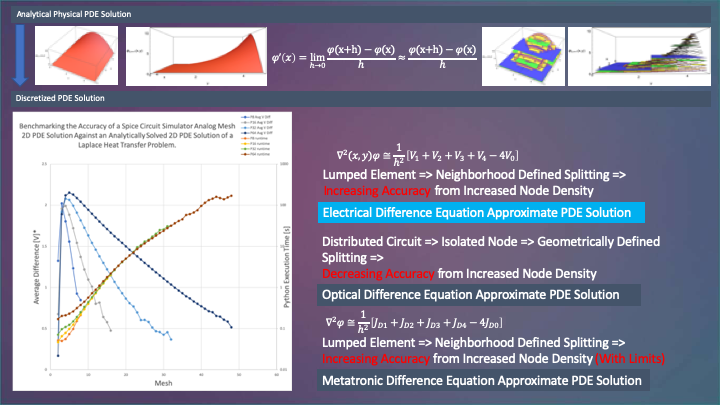
\includegraphics[height=3in, width=5.5in]{figures/figures1/03a_elec_accuracy.png}}
\caption{Electronic analog exhibits lumped element, neighborhood defined splitting, and increased accuracy from increased node density.}
\label{fig:1_03a_elec_accuracy}
\end{figure}
 
\par When transitioning from analytical to discrete Solutions, discretization error is the principal source of error in the finite difference method employed in all of the discrete information processing techniques that are discussed in the thesis. For a one dimensional problem the discretization error of $\psi$ can be defined in terms of its derivative. This spatial change is defined by $h$, and shown at the top of Figure \ref{fig:1_03a_elec_accuracy}, which is finitely small and the removal of the limit creates the approximation which is defined as the discretization error. For a dense discretized solution where the number of nodes $n$ approaches infinity and acts like a continuous solution we expect the accuracy of the overall solution to increase. One can see accuracy improvement electronically as the electronic analog exhibits lumped element, neighborhood defined splitting, and increased accuracy from increased node density as shown in Figure \ref{fig:1_03a_elec_accuracy}.

\begin{figure}[ht]
\centering\fbox{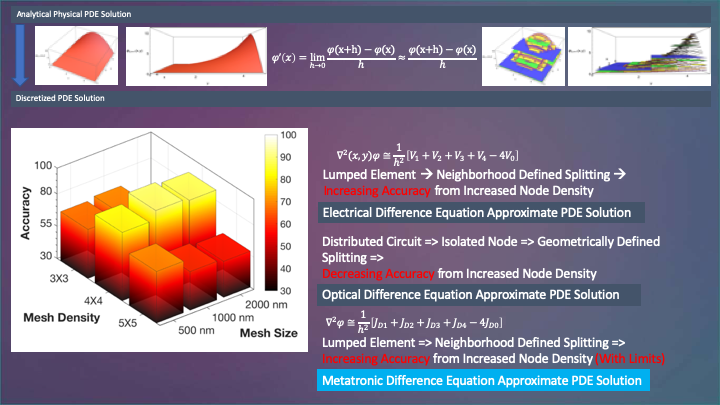
\includegraphics[height=3in, width=5.5in]{figures/figures1/03b_mt_accuracy.png}}
\caption{The metatronic circuit exhibits lumped element, neighborhood defined splitting, and therefore increasing accuracy from increased node density all at at a smaller operational wavelength than the electrical analog.}
\label{fig:1_03b_mt_accuracy.png}
\end{figure} 

\par The details of geometric optical splitting utilized in the photonics mesh is explored by my colleagues Shuai Sun and Engin Kayraklioglu who will give a deep explanation in their dissertations. However due to the distributed circuit, isolated node, and therefore geometrically defined splitting behavior, phonically one expects decreasing accuracy from increased node density. This does not mean that a photonic implementation cannot provide a useful approximate solution, but the photonic architecture needs to compensate for this negative effect. On a positive note, the metatronic circuit exhibits lumped element, neighborhood defined splitting and therefore increasing accuracy from increased node density all at at a smaller wavelength than the electrical analog as shown in Figure \ref{fig:1_03b_mt_accuracy.png}.
 






%%%%%%%%%%%%%%%%
% Chapter 2
%%%%%%%%%%%%%%%%

\chapter{Mathematics \& Physics Underlying the Computational Model}

%\acrfull{roc} is research project undertaken by a collaboration between the OPEN Lab Team under the leadership of PI Volker Sorger and the HPCL Team under the leadership of PI Tarek El Ghazawi both based at the George Washington University through the funding of an NSF RAISE Grant working to understanding the physics of, develop software for, and fabricate an analog co-processor implemented in Silicon Photonics, and Optical Metatronics, with the goal of calculating approximate solutions to 4 classes of partial differential equations comprised of Laplace, Poisson, Diffusion, and Wave. The approximate accuracy of these solutions, the time required to attain them, the energy utilized in the computation, and the physical dimension of the fabricated chip are compared against analytically derived, and numerically computed solutions, as well against a previously researched electronic analog co-processor.

\par This research is part of a larger trend punctuated by the termination of the \gls{International Technology Roadmap for Semiconductors} (\acrshort{itrs}) 2.0 report with its final 2015 publication \cite{itrs2.0_2015}. The report published for decades comprised an amalgamation of the opinions of worlds leading semiconductor researchers and industry professionals and is arguably most known for setting expectations for semiconductor \gls{technology node} scaling. However due to the challenges posed by the limits of \gls{Moore's law}, the end of \gls{Dennard scaling}, the slowing of \gls{Koomey's law}, and the limits of \gls{Amdahl's Law}. 

\par The \gls{Institute of Electrical and Electronics Engineers} (\acrshort{IEEE}) has pivoted and released the \gls{International Roadmap For Devices And Systems} (\acrshort{irds}) 2017 edition \cite{irds_2017}. In the report \acrshort{irds} acknowledges that 2D scaling will reach fundamental limits beyond 2020 and as a solution they introduce three distinct eras of scaling, Geometrical (1975-2002), Equivalent (2003 $\sim$ 2024), and 3D Power (2025 $\sim$ 2040) with Equivalent Scaling (2003 $\sim$ 2024) being defined by the "reduction of only horizontal dimension in conjunction with introduction of new materials and new physical effects". With "new vertical structures replacing planar transistors". Our research embraces this paradigm shift and falls within the scope of new materials and new physical effects. As of 2018 companies such as Xilinx have started to design processors with CPU, GPU, and FPGA architectures integrated \cite{vissers2019versal}, with the new question being which architecture is best for which task. The PDE co-processing capabilities of ROC fall within this trend.


%%%%%%%%%%%%%%%%%%%%%%%%%%  Computational Complexity  %%%%%%%%%%%%%%%%%%%%%%%%%%

\section{Computational Time Complexity Requirements}\label{bigO}
\par The two dimensional implementation of the electrical, photonic, or metatronic analog approximate \acrshort{pde} solving algorithm needs to operate as close to $O(1)$ constant time as possible in order to provide a useful analog advantage. Figure \ref{fig:2_01_computational_time_complexity} indicates the number of sources and samples needed as well as the limits of mesh dimensions in order to stay in constant time, and therefore potentially be incorporated as an analog accelerator into, as an example, the commonly used digital parallelized multi-grid method operating at a logarithmic $\Theta(\log x)$, polylogarithmic $\Theta(\log^2 x)$, or fractional Power $\Theta(\sqrt{x})$ time complexity, depending on course fine gird traversal for a grid with $x$ grid points. 

\begin{figure}[ht]
\centering\fbox{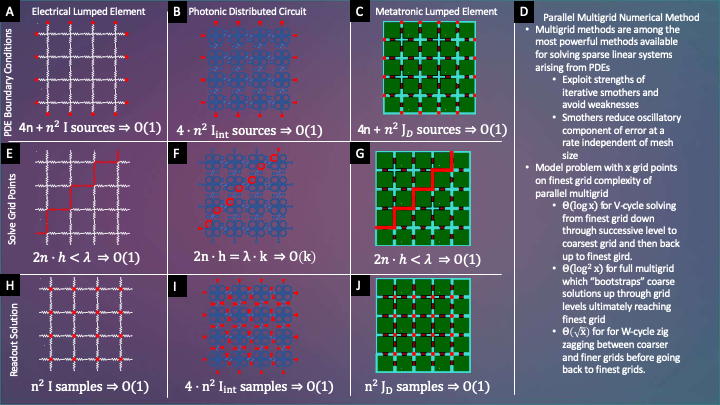
\includegraphics[height=3in,width=5.5in]{figures/figures2/01_computational_time_complexity.png}}
\caption{Computation time complexity of a single PDE analog grid solution iteration in the three analog physics technologies could be incorporated into a \textbf{(D)} parallelized  multi grid method using finite difference method operating at logarithmic time, polylogarithmic time, or fractional power time depending on the course fine grid traversal utilized. For one of the analog system to remain in the constant time domain certain hardware requirements must be met. If we assume that $n$ is the number of nodes in a one dimension side of an grid and $h$ is the length of an edge between nodes in the grid, we can see that the number of \textbf{(A)} current, \textbf{(B)} optical intensity, and \textbf{(C)} displacement current density hardware source locations are needed to set boundary conditions, shown on the top row, and we can see the needed number of \textbf{(H)} current, \textbf{(I)} optical intensity, and \textbf{(J)} displacement current density sample locations are  required to read out a PDE analog solution. With all of these sources and samples operating in parallel. The grid length scales for the \textbf{(E)} electrical \textbf{(G)} metatronic execution step remain within one operation wavelength for both technologies, and thus remain in constant time, where as the \textbf{(F)} photonic grid length scale exceeds its operational wavelength, and thus requires $k$ iterations to traverse the diameter of the grid}
\label{fig:2_01_computational_time_complexity}
\end{figure}









%%%%%%%%%%%%%%%%%%%%%%%%%%  Analytical  %%%%%%%%%%%%%%%%%%%%%%%%%%

\section{Analytical Derivation PDE Solution}\label{analyticalPDE}
\subsection{Analytical Solution}\label{analyticalSolution}

\begin{figure}[ht]
\centering\fbox{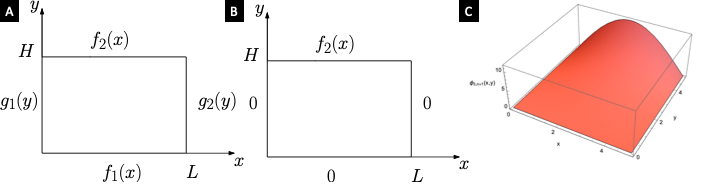
\includegraphics[height=1.5in,width=4.5in]{figures/figures2/00_analytical_pde.png}}
\caption{\textbf{(A)} The four boundaries of $\psi \left(x,y \right)$ are defined in terms of the $x$ and $y$ axis. \textbf{(B)} The one non-zero boundary condition and three zero boundary conditions for the $\varphi_3\left(x,y\right)$ solution component of $\varphi \left(x,y \right)$. \textbf{(C)} Plot of $\psi_{3,n}\left(x,y\right)$ with $n=1$, $L=5$ and $H=5$ with the continuous solution shown in the z axis.}
\label{fig:pdeBoundary}
\end{figure}

Laplace's equation is a second-order partial differential equation which produces, as a solution, harmonic functions that accurately describe the behavior of electric, gravitational and fluid potentials.  It has no time dependence, only a spatial dependence, and is often written as  

\begin{equation}\label{}
\nabla^2 \varphi = 0
\end{equation}

where \(\nabla^2\) is the Laplace operator and \(\varphi\) is a scalar function.

For the purpose of simplicity, we will only discuss spatial variables $x$ and $y$, which allows Laplace's equation to be rewritten as

\begin{equation}\label{eq:Laplace2D}
\frac{\partial^2 \varphi}{\partial x^2} + \frac{\partial^2 \varphi}{\partial y^2} = 0
\end{equation}

Following the derivation in section \ref{section:pdeDerivation} \cite{vrscay2010amath} results in the product solutions yielded by the separation of variables method up to a constant.

\begin{equation}\label{eq:sovSol_a}
\begin{aligned} 
\varphi _ { 3 , n } \left( x , y \right) & 
= \sin \left( \frac { n \pi x } { L } \right) \sinh \left(\frac { n \pi y } { L } \right)
& \text{for } n=1,2,3,\dots
\end{aligned}
\end{equation}

\subsection{Physical Units}\label{physicalUnits}
Why is necessary to discuss the physical interpretation of the purely mathematical solution of the Laplacian partial differential equation? To better understand the source of inaccuracies that deviate from the analytical solution derived in Section \ref{analyticalSolution} caused by discretization and the implementation of different analog algorithms built on physical hardware we must first address the inequality of units associated with the generated solutions. The analytical solution is purely mathematical and therefor unitless. The digitally generated discretized numerical solution outputs heat map in Kelvin [\SI{}{\kelvin}]. The electrical analog algorithm mesh can sample solutions either in Volts [\SI{}{\volt}] or current [\SI{}{\ampere}]. Photoinc ROC outputs solutions in Optical Intensity [\SI{}{\watt \meter^{-2}}]. Metatronic ROC outputs solutions in Electric Displacement Current Density $J_D$ [\SI{}{\ampere \meter^{-2}}].
\par Initially we have been normalizing all our solutions between zero and one. However to determine true equivalence in the future we can potentially add physics to our analytical solution and generate a solution for a temperature distribution in Kelvin [\SI{}{\kelvin}]. By mapping electrical, photonic ROC, and metatronic ROC to an equivalent temperature distribution in Kelvin, we can remove unit mismatch as a source of inaccuracy.

%%%%%%%%%%%%%%%%%%%%%%%%%%  Discretization  %%%%%%%%%%%%%%%%%%%%%%

\section{Discrete Numerical PDE Solution}\label{numericalPDE}
\subsection{Numerical Solution}\label{numericalSolution}

\par When using COMSOL Multiphysics to solve a two dimensional heat transfer PDE the user of the software must define the boundary conditions of the problem and specify the flux at each of those boundary conditions. This process is relatively similar to the analytical method described in Section \ref{numericalPDE}. The processes deviates when the user must specify the computational mesh element size and the geometry of the mesh showed in Figure \ref{fig:discreteSolution}. It should be noted that all computations performed in the thesis have access to the same computing resources described in Section \ref{resources}.

\begin{figure}[h]
\centering\fbox{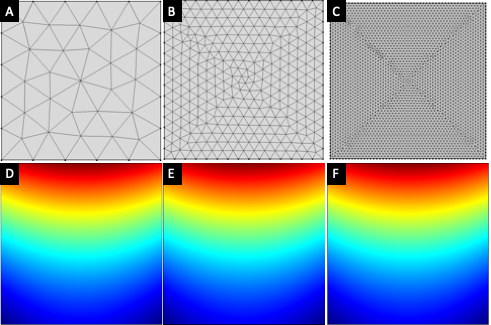
\includegraphics[height=3in,width=4.5in]{figures/figures2/01_discrete_pde.png}}
\caption{The finalized COMSOL geometry has one domain, 4 boundaries, and 4 vertices. \textbf{(A)} The physics controlled normal element size mesh consists of 68 domain elements and 20 boundary elements, \textbf{(B)} 578 domain elements and 60 boundary elements, and  \textbf{(C)} 6282 domain elements and 200 boundary elements. The number of degrees of freedom solved for is \textbf{(D)} 157 plus 44 internal DOFs and the solution is solved for in 1 seconds, \textbf{(E)} DOFs 1217 plus 124 internal DOFs solved for in 2 seconds, and \textbf{(F)} DOFs 12765 plus 404 internal DOFs solved for in 1 second.}
\label{fig:discreteSolution}
\end{figure}

\par The COMSOL Multiphyics numerical heat transfer PDE solutions are used to benchmark the accuracy of the analog algorithm implementations described in Section \ref{electricalPDE}, Section \ref{photonicPDE}, and Section \ref{metatronicPDE} because all 4 solutions include discretization error, described in Section \ref{discretizationError}, that deviates from the continuous analytical solution in Section \ref{analyticalPDE}. When striving to showcase the advantages of the analog algorithms, it is important to consider that the numerical solution benefits from the advantage of optimization of mesh geometry, shown in Figure \ref{fig:discreteSolution}, whereas the analog implementations have fixed rectangular meshes. The general lack of flexibility of analog implementations is one of there primary weaknesses, and what I try to compensate through reconfigurability.


\subsection{Discretization Error}\label{discretizationError}

\par In applied mathematics, discretization is the process of transferring continuous functions, models, variables, and equations into discrete counterparts. The discretization error is the error resulting from the fact that a function of a continuous variable is represented by a finite number of evaluations, in this case on a lattice. This visualization code for the discretization of our non physical analytical solution through the use of mesh scaling along a power law with exponent of 2 can found at \href{https://github.com/openhpclgw/roc_discrete_visualization.git}{\acrshort{roc} discrete visualization}. The discretization scaling is shown in figure \ref{fig:discrete}.

\par Discretization error is the principal source of error in the finite difference method employed in all of the information processing techniques this paper discusses. For a one dimensional problem the discretization error of $\varphi\left(x\right)$ can be defined in terms of its derivative

\begin{equation}\label{eq:discretizationError1D}
  \varphi^{\prime}\left(x\right) = \lim _ { h \rightarrow 0 } \frac { f \left( x + h \right) - f \left( x \right) } { h } \approx \frac { f \left( x + h \right) - f \left( x \right) } { h }
\end{equation}

where $h$ is finitely small and the removal of the limit creates the approximation which is defined as the discretization error. For a dense discretized solutions where the number of nodes $n$ approaches the limit $\left(2^n \Rightarrow 2^{\infty} \right)$ and acts like a continuous solution allows us to quantify the amount of inaccuracy generated by the discretization process and therefor better understand the effects of the physical properties of the electrical, optical, and metatronic information processing on their achievable accuracy's by accounting for inaccuracies caused by discretization which exists in all analog algorithm implementations.

\begin{figure}[h]
\centering\fbox{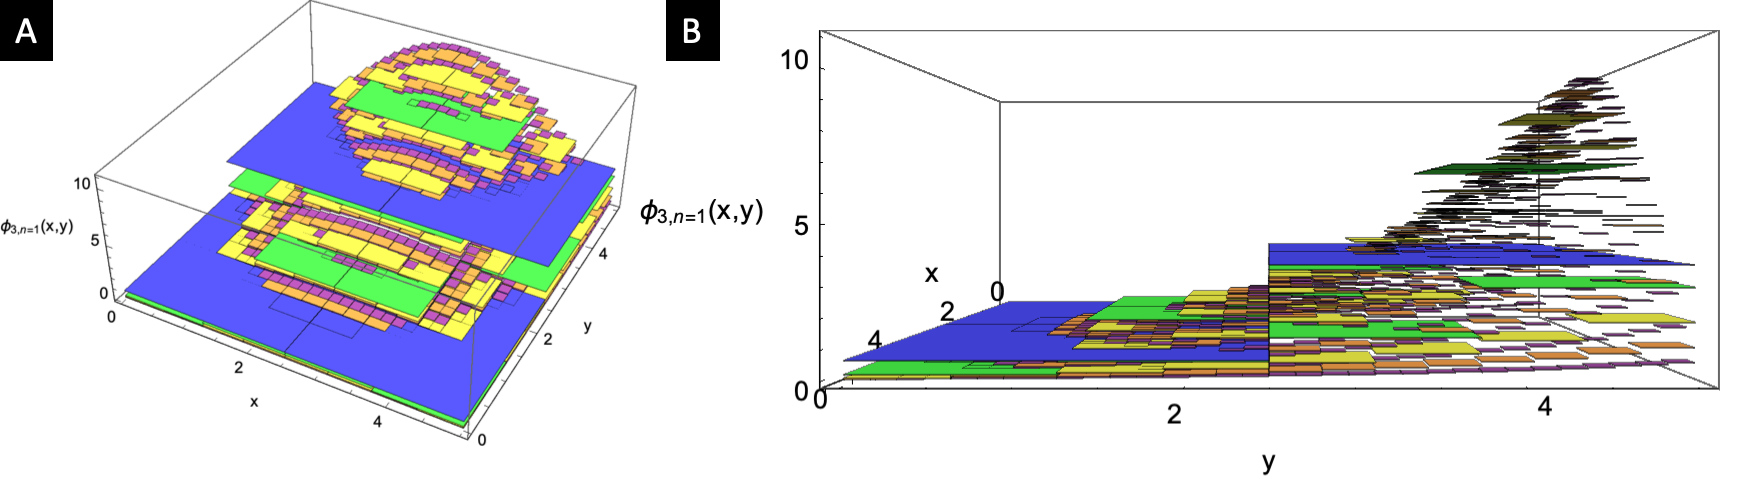
\includegraphics[height=1.5in,width=4.5in]{figures/figures2/02_discretization.png}}
\caption{\textbf{(A)} Plot of $\psi_{3,n}\left(x,y\right)$ with $L=5$ and $H=5$ with the the discretized mesh $2^1 = 2$ blue, $2^2 = 4$ green, $2^3 = 8$ yellow, $2^4 = 16$ orange, and $2^5 = 32$ purple solutions shown in the z axis. \textbf{(B)} The right side view is shown.}
\label{fig:discrete}
\end{figure}

%%%%%%%%%%%%%%%%%%%%%%%%%%  Electrical  %%%%%%%%%%%%%%%%%%%%%%%%%%

\section{Electrical Analog PDE Solution}\label{electricalPDE}
\subsection{Electrical Elements}

An electrical mesh analog finite difference algorithm utilizes basic circuit elements including capacitance (C), inductance (L), and resistance (R), from which more complex subsystems such RLC circuits can be designed. Redshaw and Liebmann designed an apparatus which uses the relaxation technique to solve PDEs describing oscillatory flow \cite{P.Palmer_1959} and heat transfer problems \cite{G.Liebmann_1950} using a resistive mesh.  This device, called a resistance network analogue, is comprised of resistors connected in a two-dimensional mesh configuration.  Finite difference mesh points characterize the stencil for a specific PDE, and are mapped to a resistive mesh for calculation.  Solutions are read at the intersection of resistor terminals, or nodes, as shown in Figure \ref{fig:electrical}.

\par This illustrates the resistance network analogue's ability to solve for a PDE using a voltage derived from current summation at each node.  Monitoring of the voltage at each node yields a solution for each element in the computational mesh.

\par Liebmann showed the error introduced by voltage and current measurements to be negligible, thus reducing the factors which limit the accuracy of the resistance network analogue to simply the mesh size and tolerance of components comprising the mesh~\cite{G.Liebmann_1950}.  Principles that govern the relaxation technique state that the mesh size must be made so small that the replacement of the PDE by the finite difference equation is permissible, and that any error introduced by a mismatch in mesh size and resolution requirement can be corrected with a correction function \cite{G.Liebmann_1950}.  Liebmann also showed that such a network of resistors contains averaging properties which minimize the error introduced by tolerances in individual resistor values \cite{G.Liebmann_1950}.

\subsection{Difference Equation Approximation}

\begin{figure}
\centering\fbox{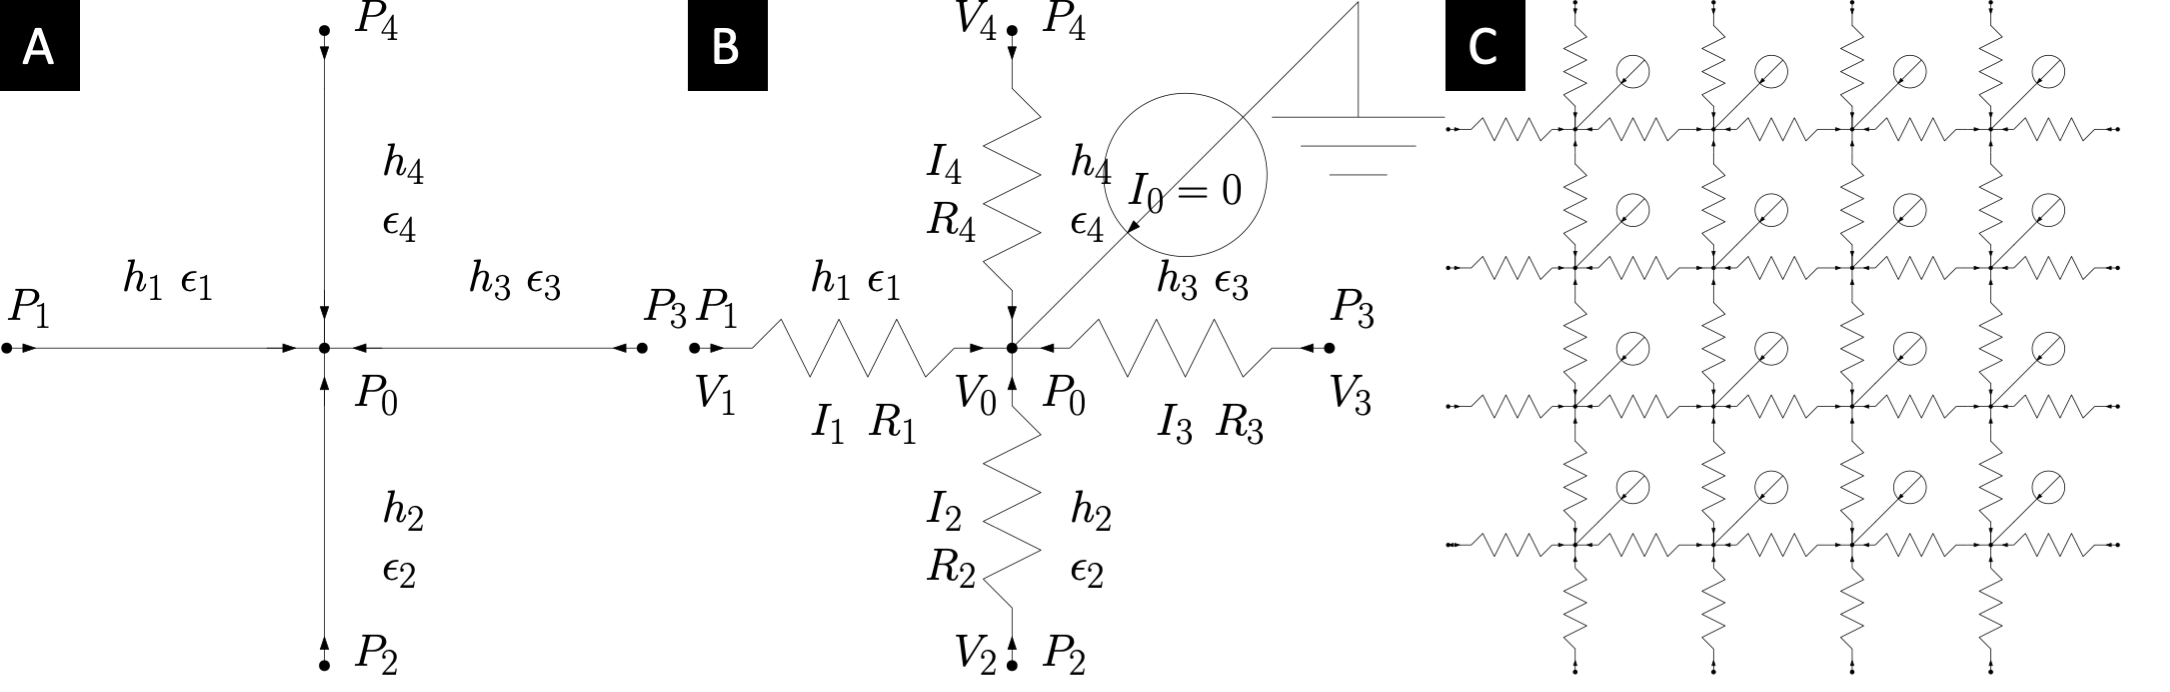
\includegraphics[height=1.5in,width=4.5in]{figures/figures2/03_finite_difference_electrical.png}}
\caption{\textbf{(A)} The derivative of the function $\varphi$ at point $P_0$ is expressed through the differences of $\varphi$ between points $P_0$ and $P_1$, $P_2$, $P_3$, and $P_4$. The distance between $P_0$ and $P_1$ is labeled $h_1$. The scalar function $\epsilon$ for vector function $\varphi$ between points $P_0$ and $P_1$, $P_2$, $P_3$, and $P_4$ is labeled $\epsilon_1$ between $P_0$ and $P_1$. \textbf{(B)}  The voltage $V$[\si{\volt}] at point $P_0$ is expressed as $V_0$. The current $I$[\si{\ampere}] and Resistance $R$[\si{\ohm}] between points $P_0$ and $P_1$ is expressed as $I_1$ and $R_1$ respectively. The same naming conventions apply for $P_2$, $P_3$, and $P_4$. $I_0$ is the input current and $R_0$ is defined in terms of other resistances, and therefor not shown on the diagram. \textbf{(C)} Poisson class electrical 16 node resistance network with the ability to apply a current at each node.}
\label{fig:electrical}
\end{figure}


\begin{equation}\label{eq:electricalLaplace_A}
  \nabla \cdot \epsilon \nabla \varphi = g 
\end{equation}

The use of an electrical mesh allows us to generate the solution of an approximation of the partial differential equation \ref{eq:supplementalElectricalLaplace} refereed to from here on as the electrical difference equation solution. In the partial difference equation \ref{eq:supplementalElectricalLaplace} where $\epsilon$ is the known scalar function, $\varphi$ is the function, and $g=0$ is  the function relationship  for a time independent Laplace second order partial differential equation. By defining an electrical mesh as shown in Figure \ref{fig:electrical} and scaling the mesh we can performing linear interpolation as shown fully in Section \ref{section:electricalDifferenceEquation} and by disregarding the higher order terms we say that Equation \ref{eq:electricalLaplace_A} is asymptotically equal to


\begin{equation}\label{eq:electricalDifferenceLaplace}
  \nabla^2 \varphi \simeq \frac{1}{h^2} \Big[ 
  \varphi\left(P_1\right) + 
  \varphi\left(P_2\right) + 
  \varphi\left(P_3\right) + 
  \varphi\left(P_4\right) -
  4\varphi\left(P_0\right)
  \Big]
\end{equation}

which is equal to

\begin{equation}\label{eq:voltageSolutionDifferenceLaplace}
  \nabla^2 \varphi \simeq \frac{1}{h^2} \Big[ V_1 + V_2 + V_3 + V_4 - 4V_0 \Big]
\end{equation}

\par The solution to the function $\varphi$ in the differential equation Equation  \ref{eq:electricalLaplace_A} has been approximated through the use of a difference equation. The solution is attained through measurement of voltage values at grid points. All that remains is to set the required boundary conditions to obtain the full solution if $g \equiv 0$ everywhere. If $g \neq 0$ currents from Equation \ref{eq:9} have to be fed into mesh points. The resistance network performs the "relaxation technique" automatically and instantaneously for a Laplace equation.

\par The accuracy of the electrical mesh pde solution is shown to increase with an increase in mesh density and be independent of the problem area size solved for between pde problem sizes 8,16,32, and 64, indicated by the reduction in the absolute (non normalized) difference between the \gls{Spice} generated electrical mesh solution script, accessible (although currently in private repository) via Section \ref{sourceCode}, and the analytical solution described in Section \ref{analyticalPDE}, and derived in Section \ref{section:pdeDerivation}, shown in Figure \ref{electricalAnalyticalDiff}. We also see that the simulation time required for the Spice circuit simulator increases exponentially for increased mesh density.

\par It is important to note that we do not have an estimate concerning the scaling of execution time of the physical electrical mesh, as we have not fabricated one, however I believe is would showcase the fundamental speedup discussed in Section \ref{bigO}. Figure \ref{electricalAnalyticalDiff} behaves in accordance with our understanding of the effects of finite difference error reduction described in Section \ref{discretizationError}.

\begin{figure}
\centering\fbox{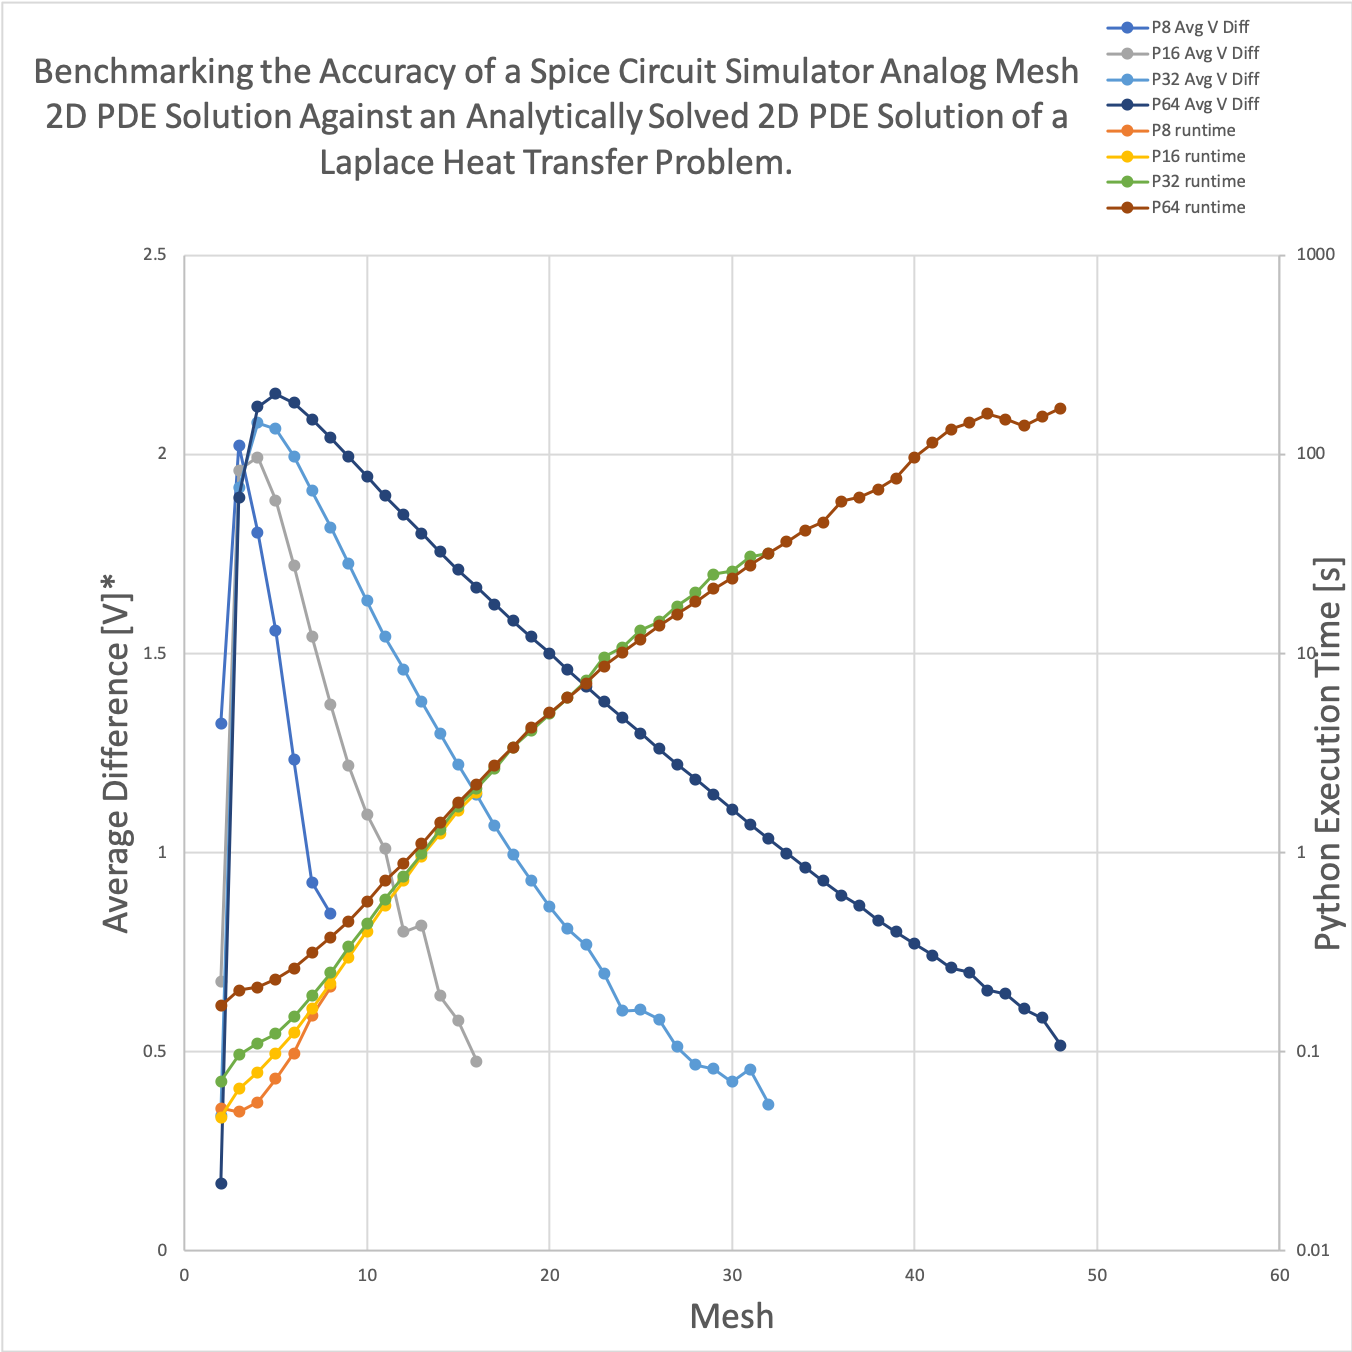
\includegraphics[height=4in,width=4in]{figures/figures2/02d_electricalDifference.png}}
\caption{Benchmarking the accuracy of a spice circuit simulator analog mesh 2D \acrshort{pde} solution against an analytically solved 2D \acrshort{pde} solution of a Laplace heat transfer problem. Mesh based solutions are scaled linearly from 2 up to the problem size N with problem sizes 8, 16, 32, and 64  plotted. Average difference is calculated by comparing the spice based voltage value at a mesh point coordinate to the value sampled from the continuous analytical solution at the same coordinate. Then the difference from all \acrfull{spice} analytical coordinate comparisons in a mesh are averaged, resulting in a single average difference point which is plotted for each mesh for each problem size. This average difference is the measure of accuracy with a higher difference resulting from a greater deviation in the spice solution from the "true north" analytical solution. Thus a lower average difference implies a higher accuracy with a value of 0 being a perfect match. *Analytical solutions not scaled for volts yet. *Program crashed at Mesh 49 on problem 64.}
\label{electricalAnalyticalDiff}
\end{figure}


%%%%%%%%%%%%%%%%%%%%%%%%%%  Photonic  %%%%%%%%%%%%%%%%%%%%%%%%%%

\section{Photonic Analog PDE Solution}\label{photonicPDE}
\par Silicon Photonics supports weighted summation through constructive and destructive interference of waveguide confined light, can be assembled into a grid/mesh structure with nodes that route light, and light sources and light detectors that are able to set boundary conditions and readout solutions. Due to these similarities it is tempting to assume an equivalence exists between the Electrical Mesh introduced in Section \ref{electricalPDE}, however we will show that there are fundamental physical differences between how the Photonic node behaves compared to the electrical node. Despite these differences Silicon Photonics has established fabrication procedures both internally at the \acrfull{open} Lab and GW \acrfull{nic} as well as externally at commercial foundries including the \acrfull{aim photonics}. The physics of Metatronic ROC discussed in Section \ref{metatronicPDE} encompass a better mapping to the Electrical Difference equation in Section \ref{electricalPDE} but current Metatronic fabrication processes are in there infancy and are currently done at length scales \cite{estakhri2019inverse} orders of magnitude greater than what is needed for our Nanoscale Metatronic ROC implementation. The combination of imperfect mapping and feasible fabrication make Photonic ROC worthy of understanding and implementing as a way to showcase current capabilities of optical analog computing. 

%\subsection{Physics of Operation}

\subsection{Limitations of Passive Photonic Difference Equation Approximation}

\par Photonic ROC operates in the optical band at $\lambda = \SI{1550}{n\meter}$ with waveguide and optical splitter dimensions in length scale order of micrometers, far larger than the operating wavelength of light, resulting in \gls{distributed element model} characteristics for the optical circuit. Current fabricated Photonic \acrshort{roc} is passive with a future active Photonic ROC planned to be fabricated at \acrshort{aim photonics}.

\par Initial experimental fabrications of Photonic ROC have been composed of pure silicon and have been \gls{passive optical} circuits, meaning that waveguide geometry is the driving force for circuit behaviour. 


\par Although there is no photonic equivalent of electrical inductance or capacitance at micrometer length scales, optical loss due to waveguide attenuation can be considered analogous to electrical current resistance. The fixed optical loss fabricated into waveguide geometries allows for passive photonic ROC to approximately solve Laplace class \acrshort{pde}s.

\par Unlike the electrical mesh, each Photonic ROC splitting node, composed of 4 ring resonators and a central splitter, due to its micrometer size and distributed element model behavior is effectively isolated from its neighborhood of surrounding nodes due to the limit of what a single wavelength of light can reach in a discrete time step. 

\par Computationally this means that at a single point in time the only physical effect that determines how much light is sent into each of three possible waveguides or is reflected back into the originating waveguide is the geometry of the node which is fixed. Irregardless of boundary conditions set and inbound light from surrounding waveguides, each optical node will always split light in the same percentages, determined by its geometry. This physics is fundamentally different from the splitting occurring in the electrical mesh in Section \ref{electricalPDE} and Metatronic ROC in Section \ref{metatronicPDE} in which each node's "visibility", due to their lumped circuit behavior, operates as an all to all network at any given time step. In a finite difference algorithm that relies on a nodes immediate neighborhood to calculate the measured value at a node, the neighborhood visibility of a single node is paramount. The effects of the photonic splitting paradigm will be explored but first it is important to understand the path that light travels through a node.

\par As light enters the node a percentage is coupled into the left and right ring resonators on either side of the waveguide prior to entering the central square where the light  is reflected off of the central circular cavity with an eventual archived splitting of roughly $33\%$ of the light traveling into each of the three surrounding waveguides as shown in Figure \ref{fig:photonic_metatronic_simulations}. The design process, physics, and geometry of this novel splitter will be covered in depth in the dissertation and future Photonic ROC fabrication paper of PhD candidate and OPEN Lab member Shuai Sun.

\begin{figure}[ht]
\centering\fbox{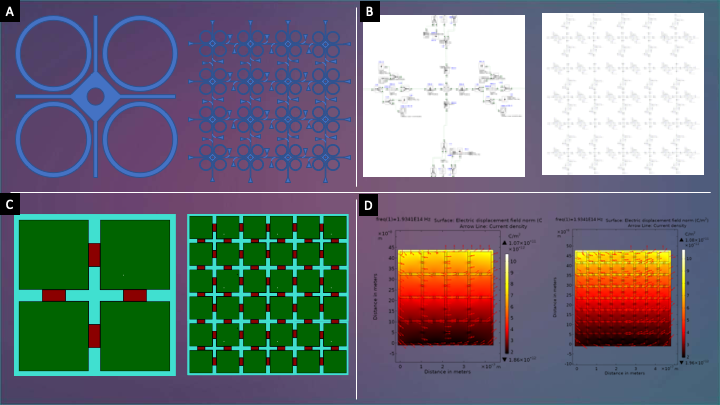
\includegraphics[height=3in, width=5.5in]{figures/figures2/04_phot_mt_models.png}}
\caption{The \textbf{(A)} geometrically engineered fixed optical loss fabricated into waveguide geometries allows for \textbf{(B)} Lumerical INTERCONNECT passive photonic \acrshort{roc} simulations to approximately solve Laplace class \acrshort{pde}s. However, unlike the electrical mesh, each photonic \acrshort{roc} splitting node, composed of 4 ring resonators and a central splitter, due to its micrometer size and distributed element model behavior is effectively isolated from its neighborhood of surrounding nodes due to the limit of what a single wavelength of light can reach in a discrete time step. The \textbf{(C)} metatronic splitting is neighborhood defined and can be \textbf{(D)} simulated with COMSOL to showcase the \acrshort{enz} confinement of displacement current density.}
\label{fig:photonic_metatronic_simulations}
\end{figure}

\par The difference equation mapping for Photonic ROC is the same as the electrical mesh up to Equation \ref{eq:3}. Once Physics becomes involved in the mapping, the first step is for current summation from the electric mesh described in Equation \ref{eq:6} to roughly map the optical intensity measured by the sum of the output grating couplers attached to each output waveguides of each splitters written as 
 
\begin{dmath}\label{eq_lightDual}
	\sum_{n=1}^{4} P_n = 0 
\end{dmath}

where $P_n$ is the optical intensity measured at each of the output grating couplers of each node.

%%%%%%%%%%%%%%%%%%%%%%%%%%  Metatronic  %%%%%%%%%%%%%%%%%%%%%%%%%%

\section{Metatronic Analog PDE Solution}\label{metatronicPDE}
\subsection{Device Physics}\label{device_physics}

\par When transitioning from the traditional static electrical resistor mesh operating in radio frequency from ($f \simeq \SI{30}{\hertz}$, $\lambda \simeq \SI{10000}{k\meter}$) to ($f \simeq \SI{300}{G \hertz}$, $\lambda \simeq \SI{1}{m\meter}$), or microwave frequency from ($f \simeq \SI{300}{M\hertz}$, $\lambda \simeq \SI{1}{\meter}$) to ($f \simeq \SI{300}{G \hertz}$, $\lambda \simeq \SI{1}{m\meter}$) described in Section \ref{electricalPDE} to the Metatronic subwavelength optical frequency domain of ($f \simeq \SI{193}{T\hertz}$, $\lambda \simeq \SI{1550}{n\meter}$) described in Section \ref{metatronicPDE}, control voltage, $V$, in each electrical node is substituted for electric field, $E$ in each Metatronic node. Thus metatronic ‘current’ is not given by the conductivity, but by the displacement current density, $J_D = \frac{\partial D}{\partial t}$, where $D$ is the electric displacement \cite{vakil2011transformation}.

\par The Metatronic circuit board needs to adhere to the condition that $J_D$ is not flowing outside the ‘wire’. This can be realized via biasing a waveguide board to the \acrfull{enz} point, where  $\text{Re}(\varepsilon)$ = real part of permittivity = 0 (or near zero). Here the ‘wire’ is given by regions where $\text{Re}(\varepsilon) >> 0$, termed \acrfull{evl}, where $J_D$ is conducted. 

\Par In order for the metatronic circuit mesh to accurately map to the finite difference equation the physical mesh dimension, $d$, must be much smaller than the optical operation wavelength, $\lambda = \SI{1550}{n\meter}$ (i.e. $d << \SI{1550}{n\meter}$) in order to create the \gls{lumped element model} condition. 

\par In order to duplicate the electrical circuit components resistors, inductors, and capacitors in the metatronic optical subwavelength domain, and in doing so reconfigure the mesh for diffusion and wave equations, the circuit must take advantage of the materials permittivity properties. If the material is a conventional dielectric (e.g., SiO2 or Si) with $\text{Re}(\varepsilon) > 0$ at optical frequencies, the nanoparticle will act as a capacitive impedance (i.e., nano capacitor). If the particle is made of material with $\text{Re}(\varepsilon) < 0$ at optical frequencies (e.g., noble metals such as Ag and Au), the particle may behave as a negatively capacitive impedance, which  implies that it will behave as an inductive impedance (i.e., nano inductor). When the material exhibits some material loss, that is when $\text{Im}(\varepsilon) \neq 0$ (which is almost always the case), a "nano resistor" element should be included in the nanocircuit \cite{N.Engheta_2007}.

\par The \acrshort{enz} materials used is \acrfull{ito} with electrical properties shown in Figure \ref{fig:ITO_material}. The \gls{Drude model} applied to ITO allows one to define optical equivalent circuit models provided the size of the mesh.

\subsection{Finite Difference Equation Equivalence}

\par Following the difference equation mapping in Section \ref{section:electricalDifferenceEquation} through Equation \ref{eq:4} and by sampling displacement current density at each node as well as the node's immediate neighborhood of nodes one edge away, we produce an asymptotically equivalent equation to partial differential equation \ref{eq:electricalLaplace_A} for each Metatronic mesh grid point

\begin{equation}\label{eq:differenceMeta}
  \nabla^2 \varphi \simeq 
  \frac{1}{h^2} \Big[ J_{D1} + J_{D2} +  J_{D3} +  J_{D4} - 4(J_{D0}) \Big].
\end{equation}

\par Equation \ref{eq:differenceMeta} is similar to the application of Kirchhoff's law to the currents $\varphi(P_i)$ meeting at the junction \textit{O} of a lumped circuit mesh described in Equation \ref{eq:voltageSolutionDifferenceLaplace}.

\begin{figure}[ht]
\centering\fbox{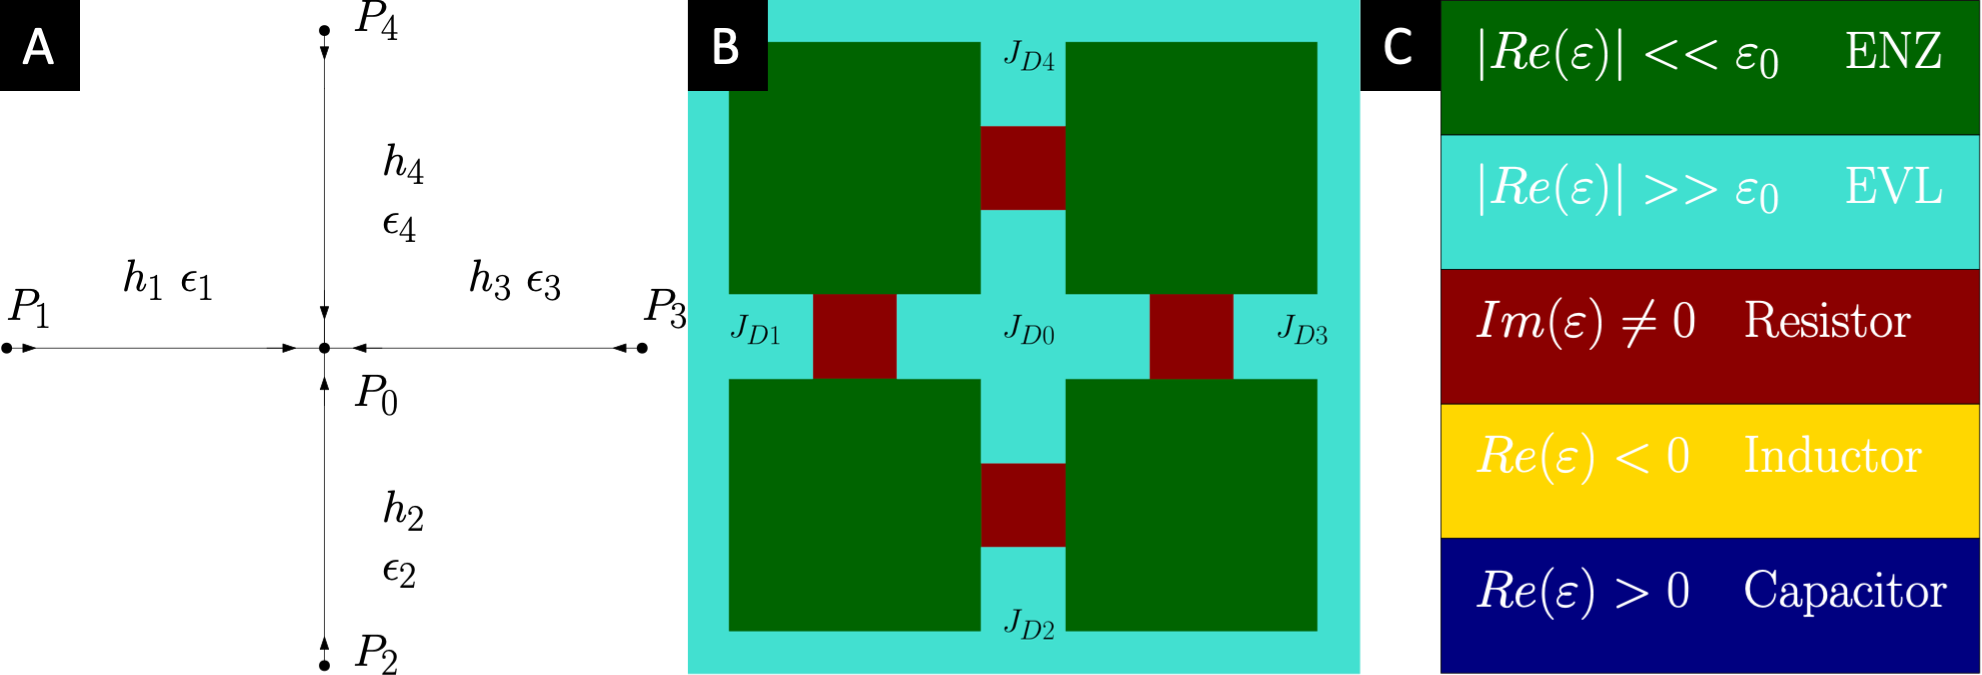
\includegraphics[height=1.5in,width=4.5in]{figures/figures2/05_finite_difference_metatronic.png}}
\caption{The figure shows a \textbf{(A)} finite difference node, a \textbf{(B)} metatronic resistive node with displacement current density sampling locations, and a \textbf{(C)} metatronic material relative permittivity reconfigurability key.}
\label{fig:metaNodeResistive}
\end{figure}

\par An equivalent metatronic nano-optic node is presented in Fig \ref{fig:metaNodeResistive}. 
We exploit the concept that nanoparticles (NPs) in the optics domain can be treated as lumped circuit elements,  whose impedance is defined in terms of the perturbation to the displacement current, $J_D$ in response of the electric field $E$. The materials complex permittivity $\widetilde{\varepsilon}$ acts as a variable for displacement current as follows

\begin{equation}
   J_D = \frac{\partial D}{\partial t} = -j \widetilde{\varepsilon} \omega E(\omega).
   \label{eq:12345}
\end{equation}

\par which, for element size considerably smaller than the optical wavelength [Engheta], represents an equivalent Ohm's law in the optical domain, enabling the mapping of the resistive circuit. In order to convey the flux of the displacement current a sub-wavelength circuit is considered to be carved in an epsilon-near-zero substrate, which for specific optical bandwidth enables light to travel through the grooves just like current in copper wiring \cite{alu2007epsilon}.

\par Resistors, capacitors and inductors can modelled as portions within the air grooves, with materials with well defined permittivity values. In order to map equation \ref{eq:7} in the metatronics circuit, the resistors are modelled as a dissipative dielectric where $R = -j\omega\widetilde{\varepsilon}$ if $\widetilde{\varepsilon}$ is a complex number. 

\par Due to the confinement of the displacement current in the air grooves, the impedances are locally coupled, which in terms of electrical circuit means that a Norton/Thevenin equivalents are admissible. Therefore, for a limited functional bandwidth, for which the material of the board is in ENZ condition, Kirchoff's law at the mesh is satisfied, providing identical results with respect to a resistive network, reported in Equation \ref{eq:differenceMeta}. 

\subsection{\label{sec:PHYSICS3} Solution of Laplace Equation}

\par By following the analytical derivation in Section \ref{section:pdeDerivation} and the electrical mesh mapping in Section \ref{section:electricalDifferenceEquation} as a starting point from which we utilizing COMSOL Multiphyiscs to simulate the electric field displacement and the displacement current in a 3x3 metatronics mesh. A strong local electric field, generated by an horizontal dipole, is used for representing the heat source, while ENZ condition is applied to the rest of the boundaries. In this section, as an illustrative and not limiting, example the permittivity of the circuit board is considered to have negligible losses ($\varepsilon''<0.1$) ($\widetilde{\varepsilon}\simeq0$) with an overall size of 1000 nm ($d<\lambda$) \cite{moitra_experimental_2014, li_-chip_2015}.

\par The overall dimension of the circuit of Fig. \ref{fig:photonic_metatronic_simulations}C is supposed to be smaller than the operating wavelength, as required for conventional electronic circuit concepts at low frequencies. However, the ‘‘spatially static-like’’ properties of the ENZ substrate, i.e. absence of a significant phase variation in ENZ, essentially relax this requirement for the optical nano-circuit board of Fig. \ref{fig:metatronic_size_simulation}, for which the total length may become also several free-space wavelengths long (while it is electrically small compared to the very long wavelength in ENZ).\cite{li_-chip_2015}

\par Under these conditions, the field lines in Figure \ref{fig:metatronic_size_simulation} highlights that the Electric displacement and consequently the displacement current, fall only within the air grooves, forced by the ENZ conditions in the neighboring area ($D\simeq0$). 

\par These COMSOL Multiphyics simulations, with maximum computational mesh size of \SI{5}{n\meter}, of electric displacement field, with $\lambda \approx \SI{1550}{n\meter} $ and $f \approx \SI{193}{T\hertz}$, over \acrfull{ito},  with complex permittivity $\epsilon = 1.0e-4 + i0.3$, in \acrfull{enz} condition squares in subwavelength optical regime surrounded by air channels, with a width of $\SI{10}{n\meter}$, broken by metatronic resistive $\SI{10}{n\meter} \times \SI{10}{n\meter}$ squares composed of \acrshort{ito} with complex permittivity $\epsilon = 1.0e-4 + i0.3$ squares described in section \ref{device_physics}. The simulation applies an initial electrical field along the top of each array with a value of $\SI{1}{\volt\meter}$ with scattering boundary conditions applied to the remaining three sides of each array. The electrical displacement current density (shown as white arrows), used to sample the \acrshort{pde} solution from the grid, is confined to the air groves surrounding and throughout the mesh.

\begin{figure}[ht]
\centering\fbox{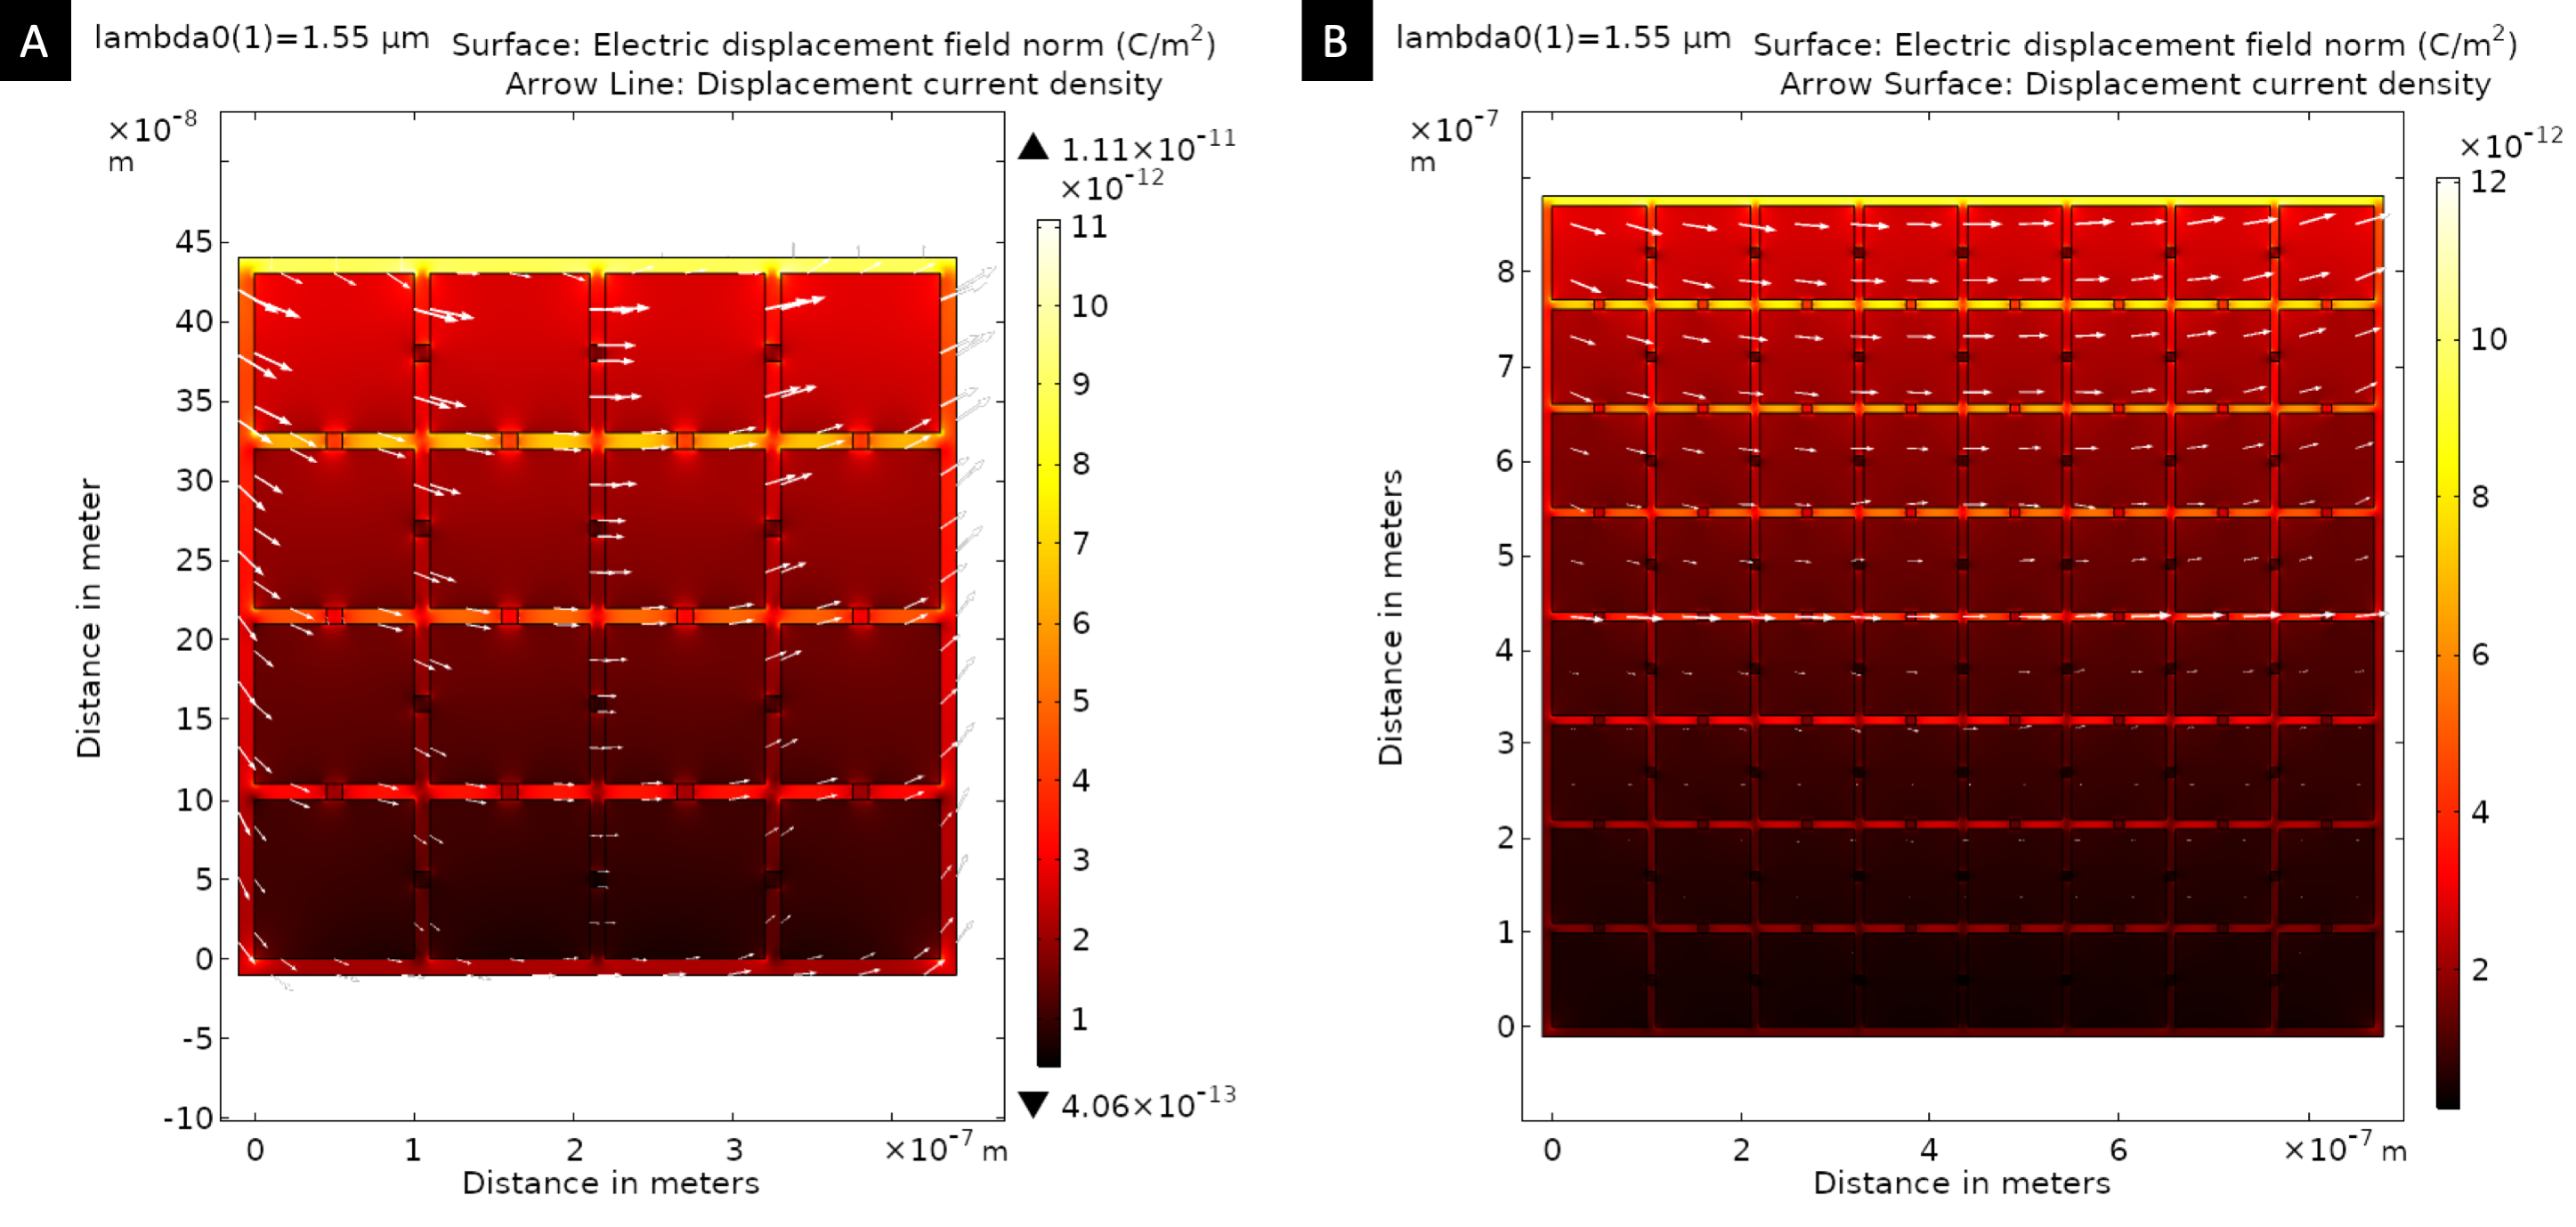
\includegraphics[width=5.5in]{figures/figures2/11_mt4_and_mt8.png}}
\caption{The \acrfull{enz} boxes in this simulation are $\SI{100}{n\meter} \times \SI{100}{n\meter}$ and the \acrfull{evl} groves are $\SI{10}{n\meter}$ wide where \textbf{(A)} contains 4 by 4 \acrshort{enz} boxes and \textbf{(B)} contains 8 by 8. One can see that at longer length scales the electric displacement field continues to produce the form of the \acrshort{pde} solution, but the containment of displacement current density within the \acrshort{evl} air groves is weakened.} 
\label{fig:metatronic_size_simulation}
\end{figure}

\par Solutions of the PDE solving metatronic processor with increasing mesh density are reported in Figure \ref{fig:metatronic_accuracy}. Interestingly, the solution given by the metatronic circuit for increasing mesh densities, keeping the overall circuit dimension, maps precisely the solution of a finer mesh in a finite difference approach.  This is can be achieved only if the circuit board is characterized by negligible losses, which causes the absence of a dielectric field displacement in the ENZ circuit board providing a perfect electric-circuit behavior. 

\par However, a study of the size and scalability and their impact on the accuracy of the solution of the metatronic processor becomes absolutely determinant if the losses in the ENZ circuit board are not negligible as discused in Section \ref{sec:ITO}). Other parameters, such as width of the grooves and smoothness of the bending curves can impact the accuracy of the solution. The undesired influence of these parameters, here not discussed,  would results in a systematic error that can be compensated or mitigated by accurate and controlled processes.

\subsection{\label{sec:ITO}  Monolythic Integration}

\begin{figure}[ht]
\centering\fbox{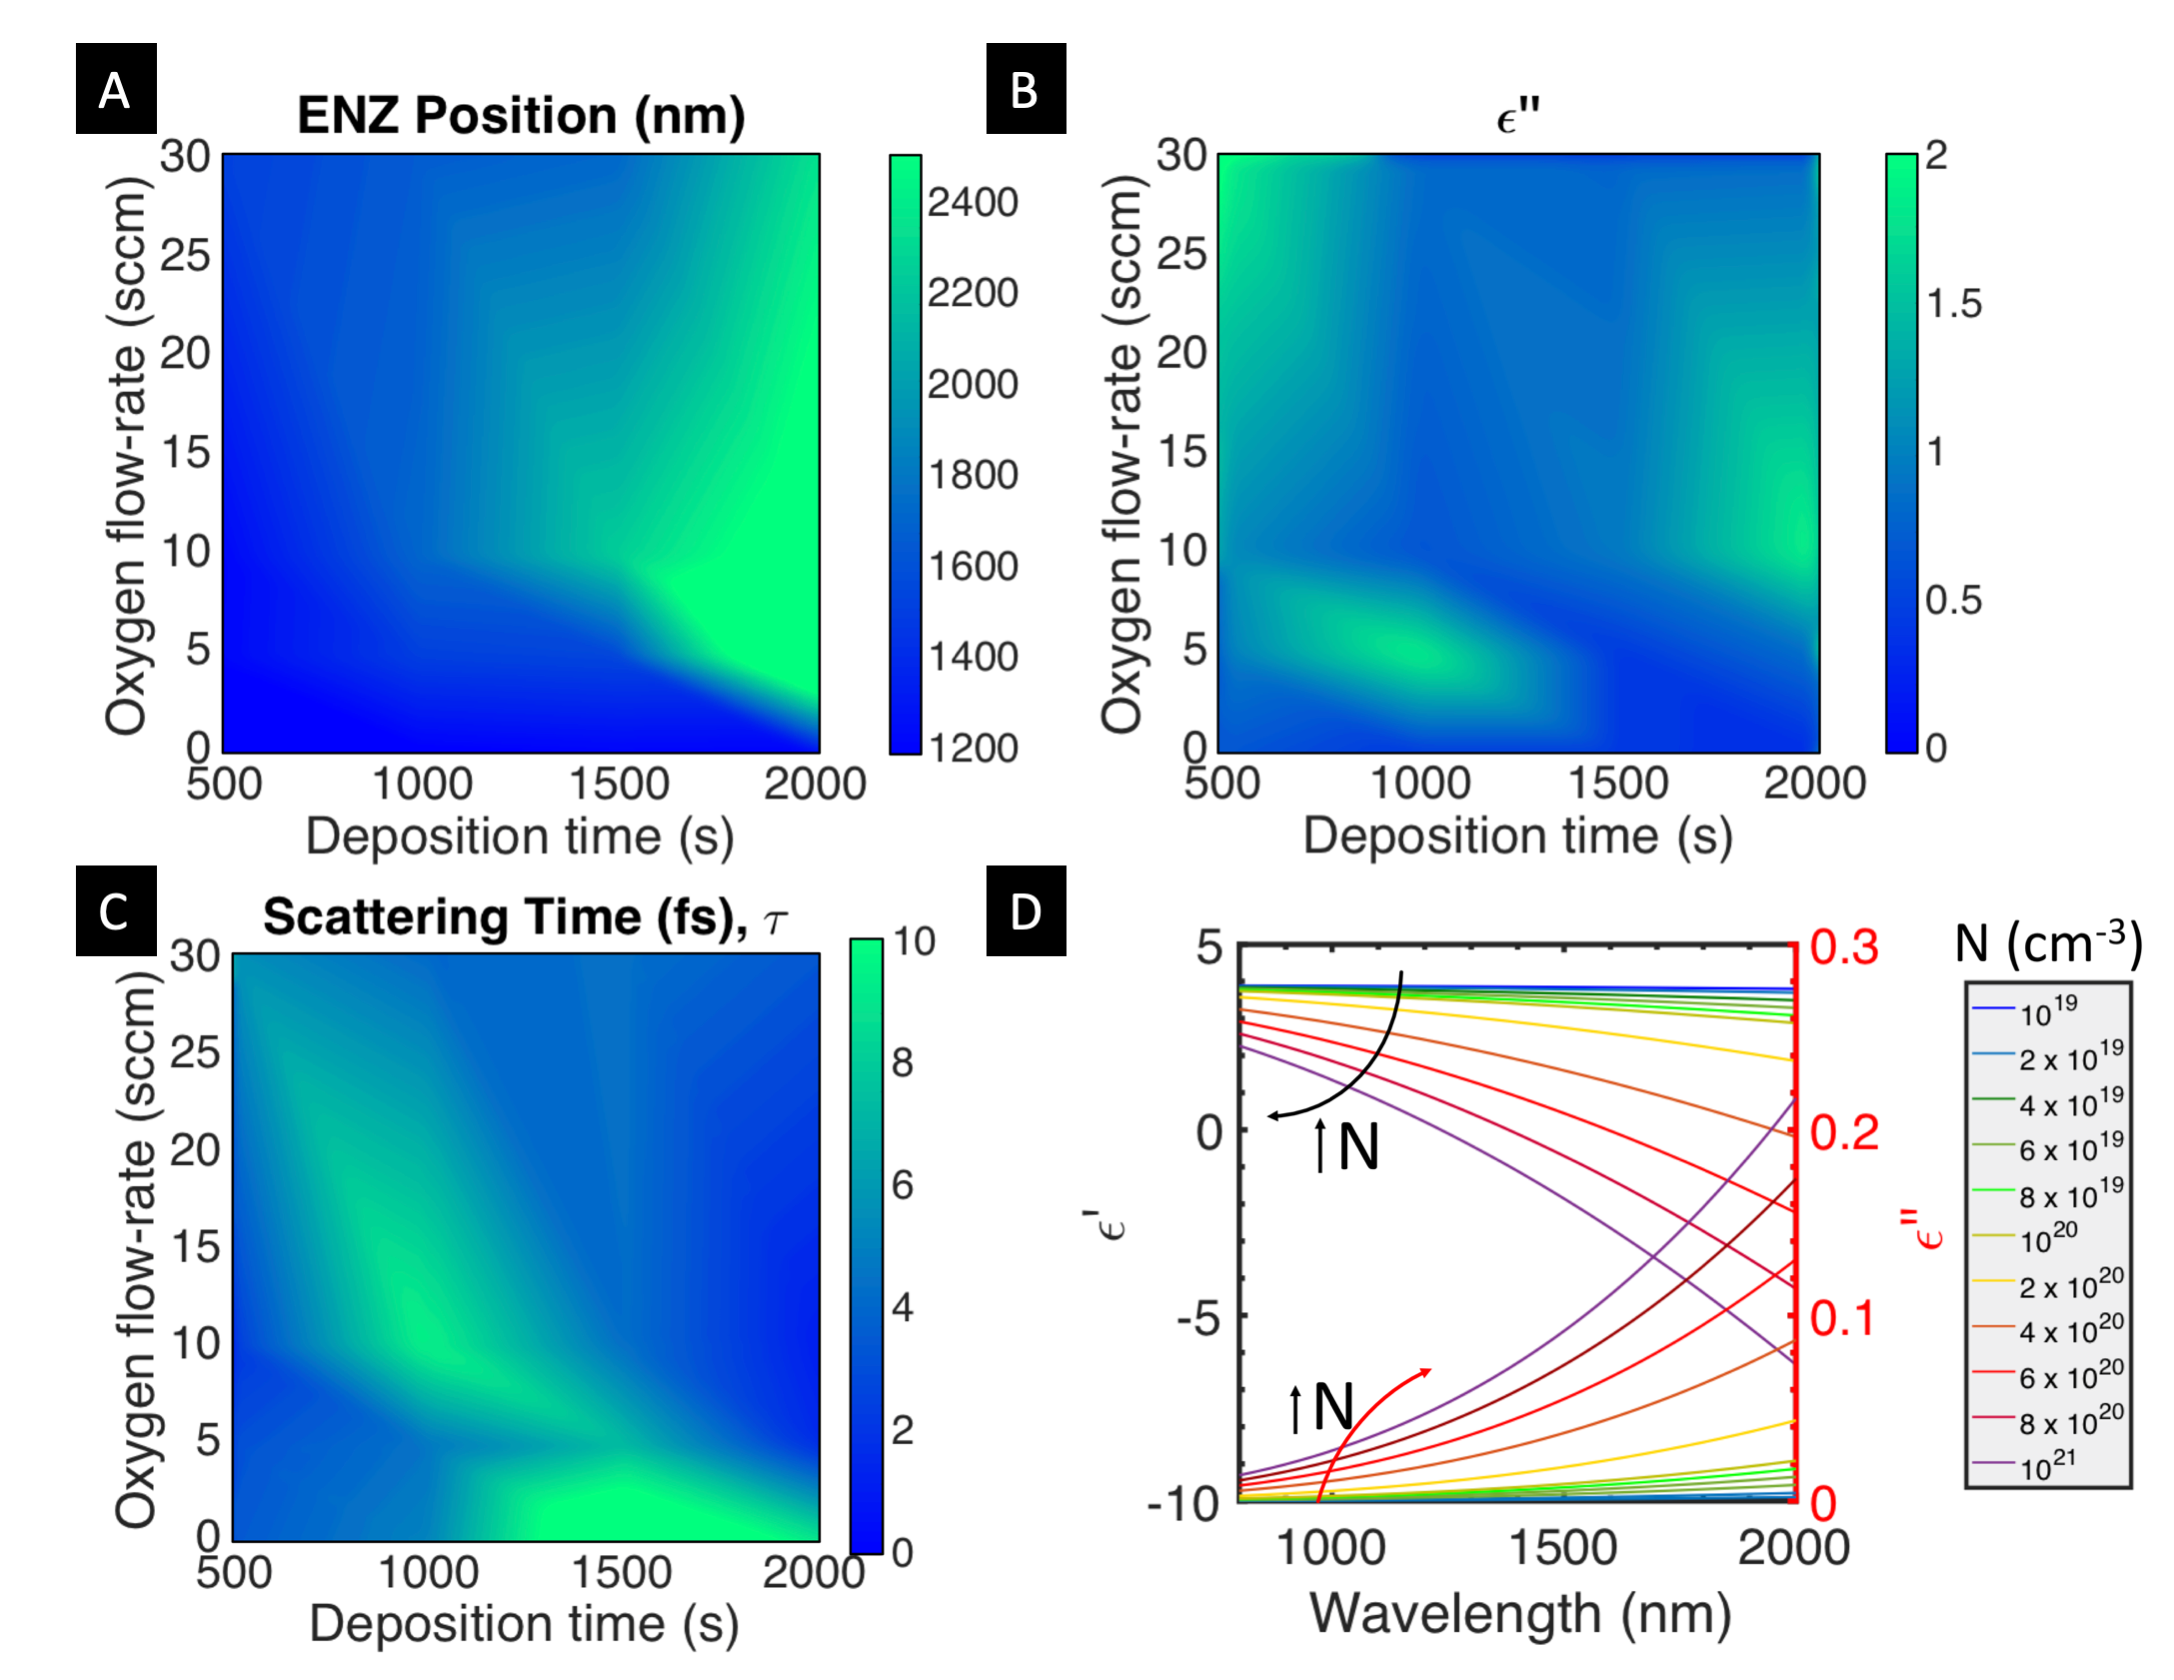
\includegraphics[width=5in]{figures/figures2/12_ito_material_new.png}}
\caption{The \textbf{(A)} ENZ wavelength, \textbf{(B)} Electrostatic doping, and \textbf{(C)} Scattering Time ($\tau_{sc}$) as function of process parameters (Oxygen flow-rate and deposition time). The  \textbf{(D)} Drude model of ITO film, sputtered with an initial electron doping of $10^{19}$cm$^{-3}$ and $\Gamma= \frac{1}{\tau_{sc}}$, for an increasing carrier modulation (blue to red).}
\label{fig:ITO_material}
\end{figure}

\par In the past years, few materials have been considered for fabricating a metatronic circuit board, such as multilayered stacks of thin film \cite{Lie1501790,PhysRevApplied.10.054021} , NPs assemblies and graphene. However, their large-scale integration is far from easy.

\par We propose Indium tin oxide as suitable material for a monolithic integration of the proposed metatronic processor. ITO has a tunable and controllable ENZ position in the NIR, according to process parameters (e.g. Oxygen flow-rate, Thermal Annealing). Its optical properties, imaginary and real part of the permittivity, can be electrostatically tuned \cite{sorger_ultra-compact_2012,amin_0.52_2018}, thus allowing GHz fast\cite{dalir_atto-joule_2018} energy efficient \cite{amin_attojoule_2018} reprogrammable features on the circuit board. 

\par Moreover, recently, our group achieved a consistent control over ITO optical parameters in particular with respect to the ENZ wavelength as function of sputtering parameter, thus allowing to bridge the technological gap in the implementation of metatronic circuits \cite{gui2018impact}. According to our fundamental studies, depicted in figure \ref{fig:ITO_material}, the ITO for the ENZ circuit board is supposed to be sputtered with 5 sccm Oxygen flow rate, enabling a 200 nm film in ENZ condition at 1550 nm, with not negligible losses $\widetilde{\varepsilon}= 0.3i$ which corresponds to a scattering time, $\Gamma= 2$ fs. The resistors, deposited using 20 sccm oxygen flow rate, which yields to $\widetilde{\varepsilon}=1.2+0.8i$  and a scattering time of 5fs. 

\par The major disadvantage is represented by the losses at ENZ condition. As a consequence of the losses in the ITO circuit board, the lines of the displacement field are not only contained in the air grooves, contrarily to the case of a ENZ material with negligible losses. In presence of non-negligible losses in the ENZ material, the circuit board is not completely insulating, since the displacement current is not negligible.

\begin{equation}
     J_D = \frac{\partial D}{\partial t}=\varepsilon"\omega E(\omega).
\end{equation}

\par There are two major kinds of phenomena that impact the accuracy of the solution, both of which depend on the ITO losses. The first one, is a function of the mesh density and the second one of the total physical length of the circuit board. High density ($>5\times5$) induces coupling within wires that shouldn't be connected, while the larger physical length ($>2\mu$m) contributes to unwanted dissipation, deviating from the original solution.

\par Figure \ref{fig:metatronic_accuracy} plots the accuracy as function of the number of nodes and physical dimension of the circuit board. The maximum accuracy ($>90$\%) is obtained for a $1\mu$m grid, with a $4\times4$ mesh density. This is achieved thanks to the trade-off between mesh size and density, which minimizes the wire coupling, without extending the wiring length, producing unwanted losses. 

\par The ITO is considered to be in a capacitor configuration, spaced by a thin dielectric, for electrostatic doping, enabling fine tuning of the permittivity values as well as updating of the problem. 

\par The variation of the carrier density via gating in ITO affects both the resistance and the ``reactance''  in the metatronics equivalent circuit, hindering the accuracy of the solution, being Imaginary, and the real part of the permittivity in Kramer-Kronig relation. Nevertheless, contrarily to the resistive circuit, if either the boundary conditions or the impedances are quickly ``refreshed'', the nano-optics equivalent circuit is substantially not affected by dispersion. In this case, the lumped circuit model still holds for high frequency modulation, since even at 100s of GHz, the timescale at which the signal is modulated does so substantially slower than the time taken by the optical signal to travel through the nano-optics network.

\subsection{\label{sec:Performance} ITO based Performance}

\begin{figure}[ht]
\centering\fbox{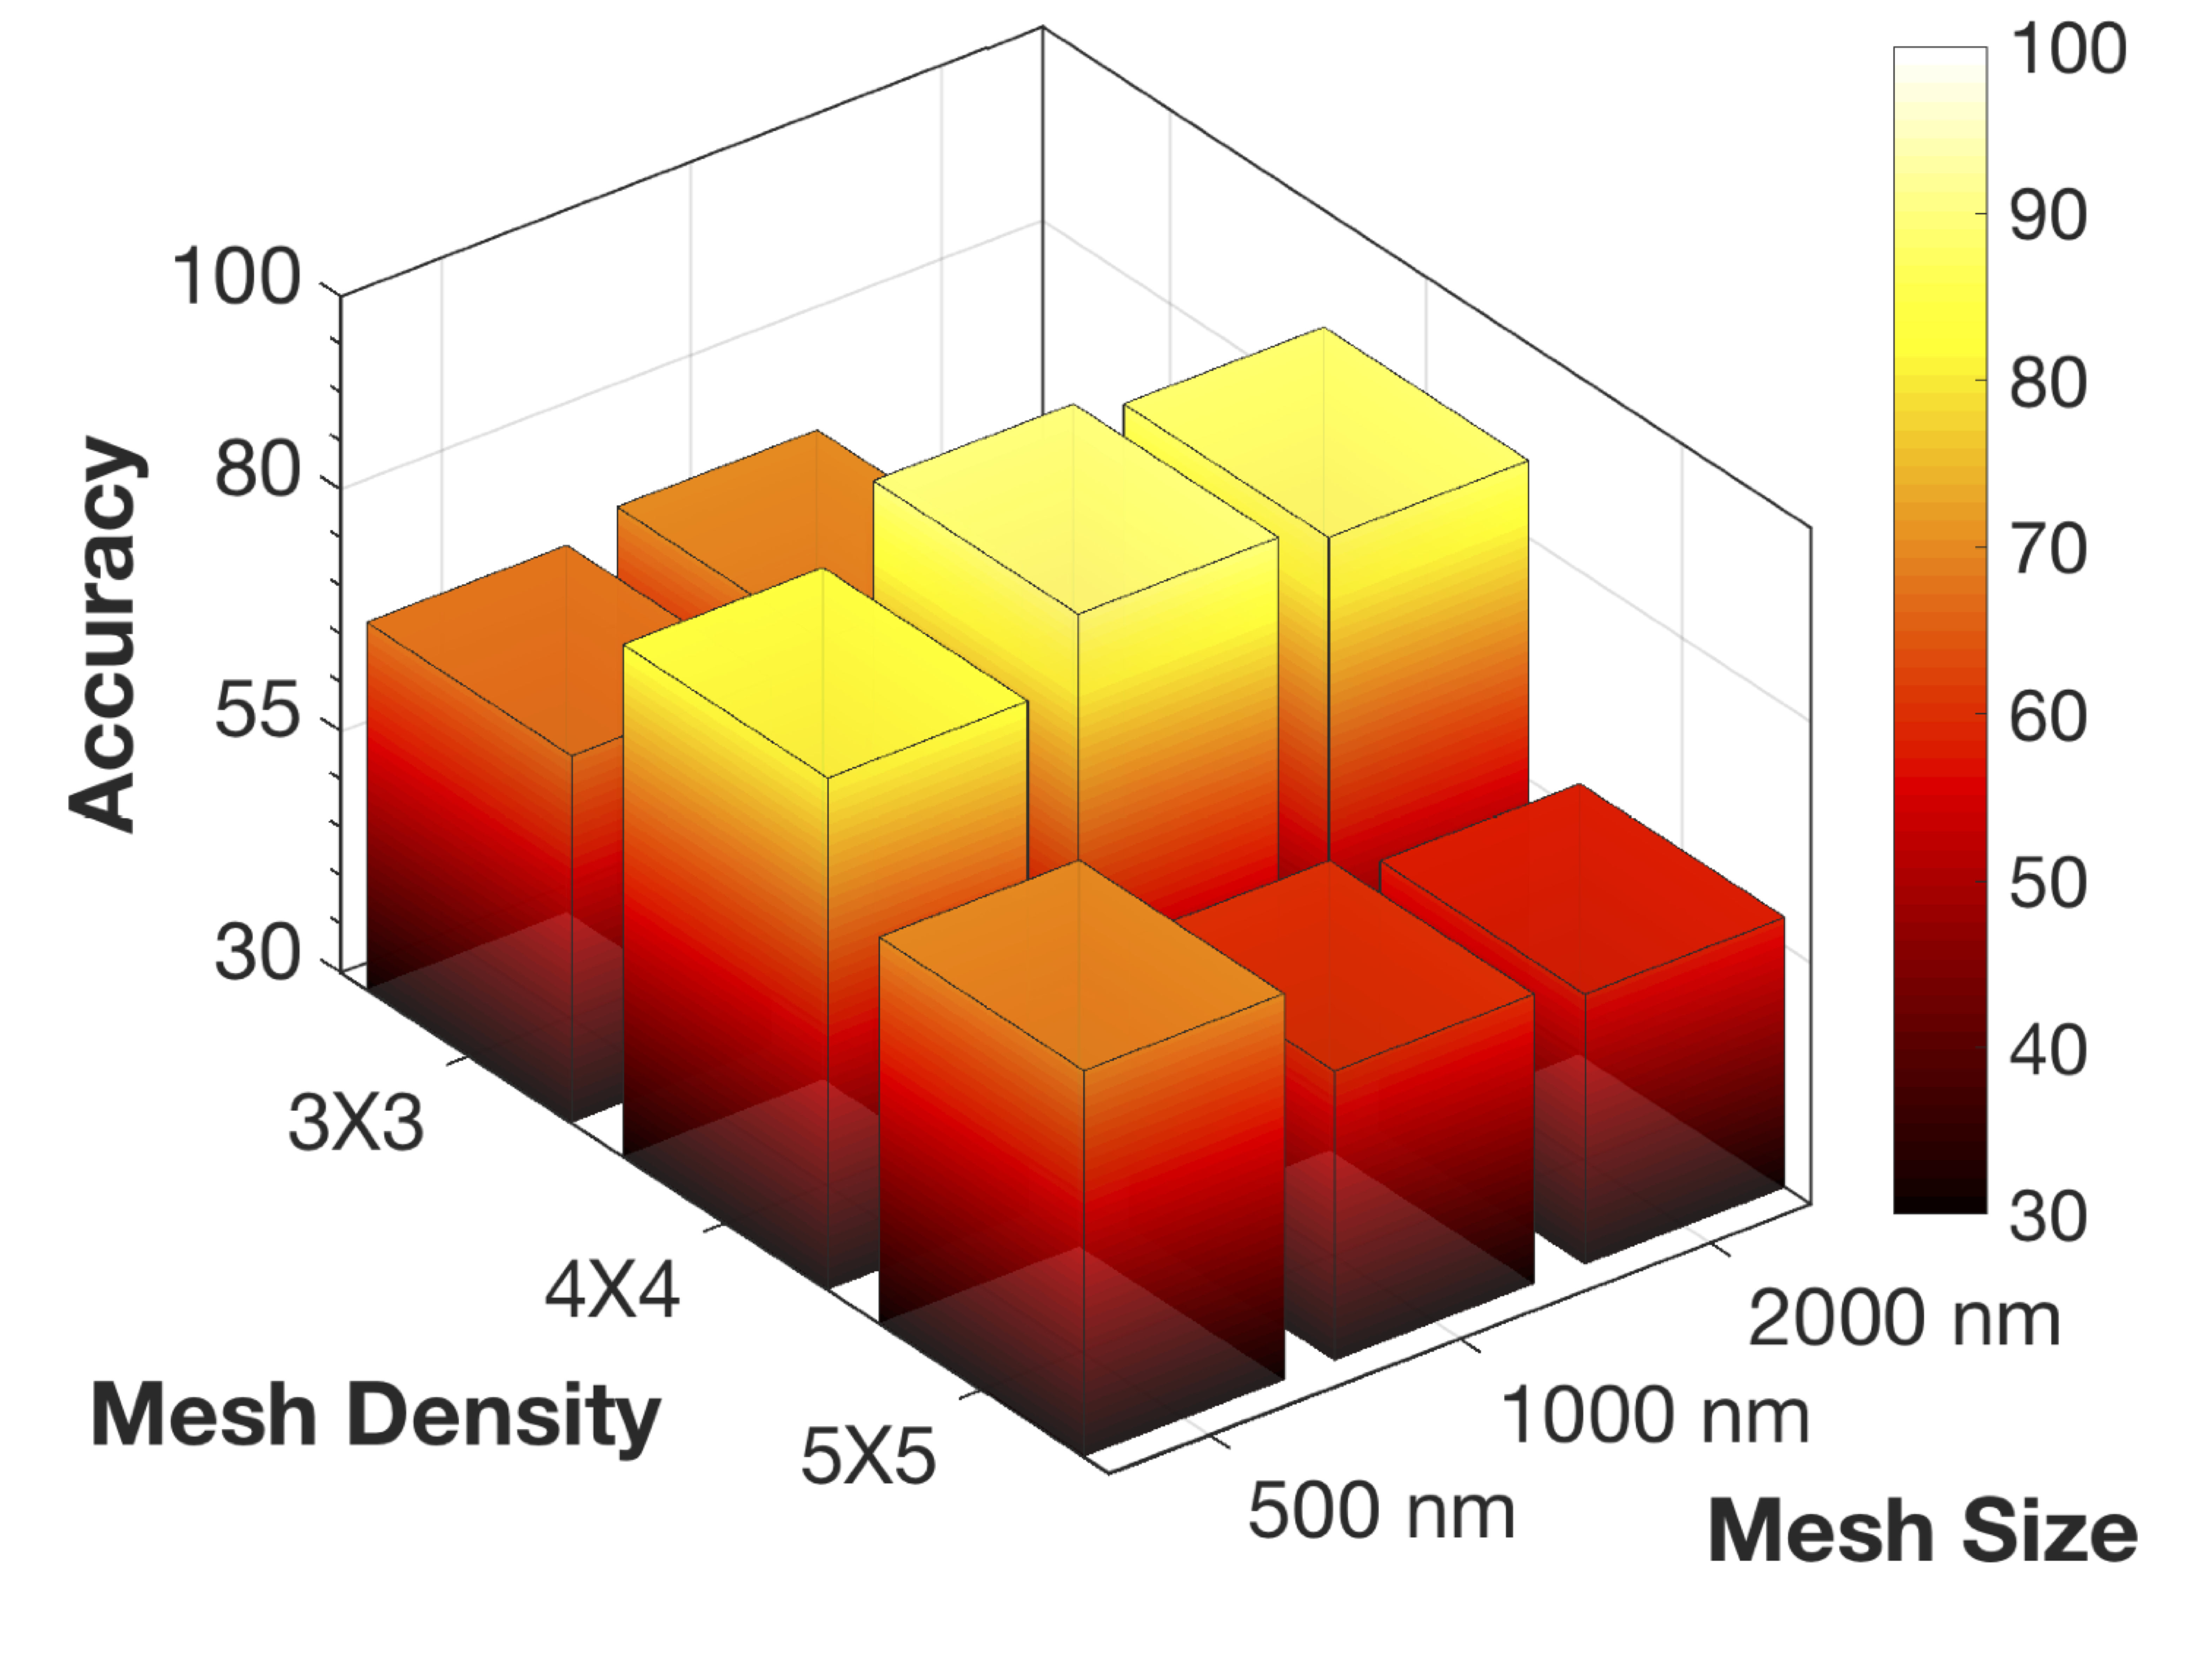
\includegraphics[width=5in]{figures/figures2/14_ito_performance_b.png}}
\caption{The metatronic solution accuracy as function of mesh density and size when compared to an discrete \acrshort{pde} solution.}
\label{fig:metatronic_accuracy}
\end{figure}

\par The main limitation of the ITO metatronic processor are the unwanted losses in the circuit board. The losses affect both the power consumption and the accuracy of the solution. However, for a small size of the processor, an approximate solution is given. The accuracy is shown in terms of error computed with respect to the solution of a finite difference of comparable mesh density.

\par The power consumption from the processor is the summation of the optical power used for exciting the dipole (initiating the processor) and the the radio frequency power employed for modulating the carrier densities of each lumped elements, i.e. reprogramming the circuit. Concerning the reconfigurability of the processor, recent works showed attojoule efficient \cite{amin_attojoule_2018,dalir_atto-joule_2018} ITO based modulators operating at high speed. On the other hand, few mW optical power are needed for exciting the fluorescent molecule and setting the boundary conditions. Although, efficient measurements schemes must be used for detecting the electric field displacement at each node of the metatronic mesh, avoiding scanning over the sample, e.g. high resolution tip enhanced near field spectroscopy, in order to minimize the power used for the detection mechanism.

\subsection{\label{sec:Probe} Near Field Displacement Measurement}

\begin{figure}[h]
\centering\fbox{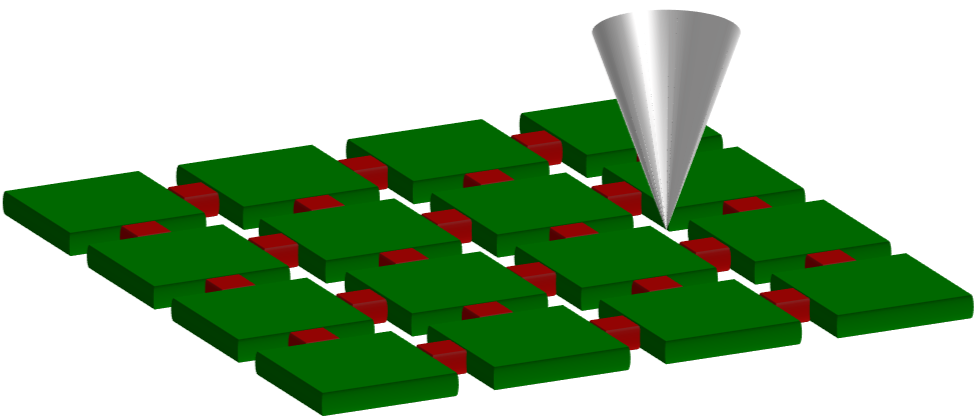
\includegraphics[width=4in]{figures/figures2/15_probetip.png}}
\caption{Schematic representation of a "Nanophotonic Probe". An impinging radiation excites a fluorescent molecule, creating a local near field, which produces an electric displacement in the metatronic circuit. The displacement is probed by the tips of a probe card, in a campanile tip aperture nSOM configuration.}
\label{fig:nanophotonic_probe}
\end{figure}

\par In order to sample the electric field displacement signal at the nodes of the metatronic mesh, deep sub-wavelength near field microscopy has to be employed with nanometric spatial resolution \cite{bao_mapping_2012,bao_visualizing_2015,caselli_deep-subwavelength_2015}. Although, regular Near-field is associated with AFM systems, thus requiring long scanning time. In this section, we propose a Nano-optic probe card for reading of the values of the local displacement field as shown in Figure \ref{fig:nanophotonic_probe}). The reading mechanism is based on multiple tips characterized by sub-wavelength aperture at the apex which collects the local near field radiation similarly to a local near field microscope, allowing for a parallel reading out. NSOM would be preferential with respect to Scattering type SNOM since the former will minimize the coupling between vertical dipoles, i.e. metallic tip, introducing second order scattering and a higher degree of uncertainty in the system.





%%%%%%%%%%%%%%%%%%%%%%%%%%  Supplemental  %%%%%%%%%%%%%%%%%%%%%%%%%%

\section{Supplemental Material}

\subsection{Analytical Solution to a Laplacian Steady State Heat Transfer PDE}\label{section:pdeDerivation}


Laplace's equation is a second-order partial differential equation which produces, as a solution, harmonic functions that accurately describe the behavior of electric, gravitational and fluid potentials.  It has no time dependence, only a spatial dependence, and is often written as  

\begin{equation}\label{eq:supplementalLaplace}
\nabla^2 \varphi = 0
\end{equation}

where $\nabla^2$ is the Laplace operator and $\varphi$ is a scalar function.

For the purpose of simplicity, we will use Cartesian coordinate system and only discuss spatial variables $x$ and $y$, which allows Laplace's equation to be rewritten as

\begin{equation}\label{eq:supplementalLaplace2D}
\frac{\partial^2 \varphi}{\partial x^2} + \frac{\partial^2 \varphi}{\partial y^2} = 0
\end{equation}

which is equivalent to equation \ref{eq:supplementalLaplace} for two dimensions. We are therefor solving a second order linear PDE. This describes a steady state system, and can be used for: 

\begin{itemize}
  \item steady state temperature distributions
  \item steady state stress distributions
  \item steady state potential distributions
  \item steady state flows
\end{itemize}

We will evaluate the problem over the rectangular region $0 \leq x \leq L$, $0\leq y \leq H$ for a fixed boundary temperature distribution.

\begin{equation}\label{eq:supplementalBoundaryFunction}
\begin{split}
\varphi \left( x , 0 \right) & = f _ { 1 } \left( x \right) \\ 
\varphi \left( L , y \right) & = g _ { 2 } \left( y \right) \\ 
\varphi \left( x , H \right) & = f _ { 2 } \left( x \right) \\ 
\varphi \left( 0 , y \right) & = g _ { 1 } \left( y \right)
\end{split}
\end{equation}

The four fixed boundary temperature distributes are non homogeneous, meaning that we cannot apply the  separation of variables technique to solve the problem. However we can divide $\varphi \left(x,y \right)$ into its four components, where each component $\varphi_i$ will satisfy one non-zero boundary condition and three zero boundary conditions. 

\begin{equation}\label{eq:supplementalFourComponents}
\begin{split}
\varphi \left( x , y \right) = \varphi _ { 1 } \left( x , y \right) + \varphi _ { 2 } ( x , y ) + \varphi _ { 3 } \left( x , y \right) + \varphi _ { 4 } \left( x , y \right)
\end{split}
\end{equation}

With this in mind we will set our non-zero boundary condition to be at the top of our problem which will act as a heat source when we compare our analytical result to our electrical and optical solutions.


\begin{equation}\label{eq:supplementalOneNonZero}
\begin{array} {c c c c} 
{ \mathrm { BC1 } : } & { \varphi _ { 3 } \left( x , 0 \right) = 0 } & { \mathrm { for } } & { 0 \leq x \leq L} \\ 
{ \mathrm { BC2 } : } & { \varphi _ { 3 } \left( L , y \right) = 0 } & { \mathrm { for } } & { 0 \leq y \leq H} \\ 
{ \mathrm { BC3 } : } & { \varphi _ { 3 } \left( x , H \right) = f _ { 2 } \left( x \right) } & { \mathrm { for } } & { 0 \leq x \leq L} \\ 
{ \mathrm { BC4 } : } & { \varphi _ { 3 } \left( 0 , y \right) = 0 } & { \mathrm { for } } & { 0 \leq y \leq H} 
\end{array}
\end{equation}

Now we can apply separation of variables to each $\varphi_i$ function. For $\varphi_3 \left(x,y \right)$ we set the following

\begin{equation}\label{eq:supplementalSov}
\begin{split}
\varphi _ { 3 } \left( x , y \right) = X \left( x \right) Y \left( y \right)
\end{split}
\end{equation}

The three homogeneous boundary conditions will yield the following conditions 

\begin{equation}\label{eq:supplementalSovThreeZero}
\begin{array} { c c c c } 
{ \mathrm { BC1 } : } & { X\left(x\right)Y\left(0\right)= 0 } & { \Rightarrow } & { Y\left(0\right) = 0} \\ 
{ \mathrm { BC2 } : } & { X\left(L\right)Y\left(y\right) = 0 } & { \Rightarrow }  & { X\left(L\right) = 0} \\ 
{ \mathrm { BC4 } : } & { X\left(0\right)Y\left(y\right) = 0 } & { \Rightarrow } & { X\left(0\right) = 0} \end{array}
\end{equation}

Substitution of \ref{eq:supplementalSov} into \ref{eq:supplementalLaplace2D} yields

\begin{equation}\label{eq:supplementalSovLaplace2D}
X ^ { \prime \prime } \left( x \right) Y \left( y \right) + X \left( x \right) Y ^ { \prime \prime } \left( y \right) = 0
\end{equation}

which is separated into

\begin{equation}\label{eq:supplementalSovk}
\frac{X''\left(x\right)}{X\left(x\right)} = -\frac{Y''\left(y\right)}{Y\left(y\right)} = k
\end{equation}

where k is a constant equal to, greater than, or less then zero. The separation yields the following problems  for $X$ and $Y$

\begin{equation}\label{eq:supplementalSovX}
X\left(x\right) ^ { \prime \prime } - k X\left(x\right) = 0 , \quad X \left( 0 \right) = X \left( L \right) = 0
\end{equation}

and

\begin{equation}\label{eq:supplementalSovY}
Y\left(y\right) ^ { \prime \prime } + k Y\left(y\right) = 0 , \quad Y \left( 0 \right) = 0
\end{equation}

For $X(x)$ we now need to find if a nontrivial solution exists for a value of k
\begin{enumerate}
  \item Case $k>0$
  \begin{enumerate}
  	\item Boundary Value Problem: $X(x)^{\prime\prime}-kX(x)=0$, $X(0)=X(L)=0$
  	\item General Solution: $X(x) = C_1 e^{\sqrt{k}x} + C_2 e^{-\sqrt{k}x}$
    \item Boundary Condition: $X(0) = 0$ implies that $C_1 + C_2 = 0$, or $C_2 = -C_1$, so that $X(x)=C_1 [e^{\sqrt{k}x} - e^{-\sqrt{k}x}  ] = 2C_1 \sinh ( \sqrt{k}x )$
    \item Boundary Condition: $X(L) = 0$ implies that $C_2\sinh (\sqrt{k}L) = 0$, which is satisfied only if $C_2 =0$. This follows from the fact that $\sinh(x)$ is zero only at $x = 0$.  
    \item Trivial Solution: The only solution to the boundary value problem for $k>0$ is the trivial solution $X(x)=0$.
  \end{enumerate}
  \item Case $k = 0$
  \begin{enumerate}
  	\item Boundary Value Problem: $X(x)^{\prime\prime}=0$, $X(0)=X(L)=0$
  	\item General Solution: $X(x)=C_1x+C_2$
    \item Boundary Condition: $X(0)=0$ implies that $C_2 = 0$. 
    \item Boundary Condition: $X(L)=0$ implies that $C_1L = 0$, or $C_1 = 0$.  
    \item Trivial Solution: The only solution to the case $k=0$ is $X(x) = 0$ 
  \end{enumerate}
  \item Case $k<0$
  \begin{enumerate}
  	\item Boundary Value Problems: $X(x)^{\prime\prime}-kX(x)=0$, $X(0)=X(L)=0$
  	\item Define: $k = -\lambda$ so the $\lambda > 0$
  	\item General Solution: $X(x) = C_1\cos(\sqrt{\lambda}x) + C_2\sin(\sqrt{\lambda}x)$
    \item Boundary Condition: $X(0) = 0$ implies that $C_1 + C_2 \cdot 0 = 0$ which implies that $C_1 = 0$
    \item Boundary Condition: $X(L) = 0$ combined with $X(x)=C_2\sin(\sqrt{\lambda}x)$ implies that $\sin(\sqrt{\lambda}L) = 0$
  \end{enumerate}
\end{enumerate}

A nontrivial solution exists for $k<0$. Since $L$ is fixed, we must adjust $\lambda$ in order that the above equation is satisfied. We set $k=-\lambda$, where $\lambda > 0$ gives

\begin{equation}\label{sovXLambda}
X\left(x\right) ^ { \prime \prime } + \lambda X\left(x\right) = 0 , \quad X \left( 0 \right) = 0 , \quad X \left( L \right) = 0
\end{equation}

with eigenvalues of 

\begin{equation}\label{eigen}
\lambda = \lambda _ { n } = \left( \frac { n \pi } { L } \right) ^ { 2 } , \quad n = 1,2,3 , \cdots
\end{equation}

and associated eigenfunctions

\begin{equation}\label{eigenfunction}
X _ { n } \left( x \right) = \sin \left( \frac { n \pi } { L } \right)
\end{equation}

Now consider the $Y$ equation while recalling that $k=-\lambda$ so that $k_n = -\lambda_n$. The associated $Y_n$ function will satisfy the differential equation

\begin{equation}\label{eq:ivpY}
Y\left(y\right) ^ { \prime \prime } - \left( \frac{n\pi}{L} \right)^2 Y\left(y\right) = 0 , \quad Y \left( 0 \right) = 0
\end{equation}

Equation \ref{eq:ivpY} is not longer a boundary value problem but is now an initial value problem with only one condition. The general solution can be written as

\begin{equation}\label{eq:ivpYGS}
Y_{ n } \left( y \right) = A _ { 1 } e ^ { n \pi y / L } + A _ { 2 } e ^ { - n \pi y / L }
\end{equation}

but it is more convenient to use a hyperbolic functions

\begin{equation}\label{eq:ivpYGSHyper}
Y _ { n } \left( y \right) = B _ { 1 } \cosh \left( \frac{n \pi y} { L } \right) + B _ { 2 } \sinh \left(\frac{ - n \pi y }{ L }\right)
\end{equation}

The condition $Y \left( 0 \right) = 0$ implies that $B_1 = 0$ This is due to the fact that $\cosh \left(0\right) = 1$ and $\sinh \left(0\right) = 0$. Therefor for $Y_n(0)$ to equal $0$, $B_1$ must equal $0$. This shows that the $Y_n \left(y\right)$ function associated with the $X_n \left(x\right)$ function is

\begin{equation}\label{eq:ivpYSol}
Y _ { n } \left( y \right) =  B _ { 2 } \sinh \left(\frac{ - n \pi y }{ L }\right)
\end{equation}

This results in the product solutions yielded by the separation of variables method up to a constant.

\begin{equation}\label{eq:sovSol}
\begin{aligned} 
\varphi _ { 3 , n } \left( x , y \right) & = X _ { n } \left( x \right) Y _ { n } \left( y \right) 
= \sin \left( \frac { n \pi x } { L } \right) \sinh \left(\frac { n \pi y } { L } \right)
& \text{for } n=1,2,3,\dots
\end{aligned}
\end{equation}

\subsection{Mapping of Difference Equation Approximation to Electrical Resistance Mesh}\label{section:electricalDifferenceEquation}


\begin{equation}\label{eq:supplementalElectricalLaplace}
  \nabla \cdot \epsilon \nabla \varphi = g 
\end{equation}

The use of an electrical mesh allows us to generate the solution of an approximation of the partial differential equation \ref{eq:supplementalElectricalLaplace} refereed to from here on as the electrical difference equation solution. In the partial difference equation \ref{eq:supplementalElectricalLaplace} where $\epsilon$ is the known scalar function, $\varphi$ is the function, and $g=0$ is  the function relationship  for a time independent Laplace second order partial differential equation. By performing \gls{linear interpolation} on Figure \ref{fig:electrical} and disregarding the higher order terms we say that Equation \ref{eq:supplementalElectricalLaplace} is asymptotically equal to:

\begin{equation}\label{eq:2}
\begin{split}
  \nabla \cdot \epsilon \nabla \varphi \simeq \\
  &\quad 
  \frac{2}{h_1 + h_3} 
  \Big[ 
  	\frac{\epsilon_1}{h_1} ( \varphi(\vec{P_1}) - \varphi(\vec{P_0})) 
  +
  	\frac{\epsilon_3}{h_3} ( \varphi(\vec{P_3}) - \varphi\vec{P_0})) 
  \Big]\\
  &\quad
  + 
    \frac{2}{h_2 + h_4} 
  \Big[ 
  	\frac{\epsilon_2}{h_2} ( \varphi(\vec{P_2}) - \varphi(\vec{P_0})) 
  +
  	\frac{\epsilon_4}{h_4} ( \varphi(\vec{P_4}) - \varphi(\vec{P_0})) 
  \Big] 
\end{split}
\end{equation}

By setting neighboring points equal distant $h = h_1 = h_2 = h_3 = h_4$ and having a constant scalar function $\epsilon = \epsilon_1 = \epsilon_2 = \epsilon_3 = \epsilon_4$

\begin{equation}\label{eq:3}
\begin{split}
  \nabla \cdot \epsilon \nabla \varphi \simeq \\
  &\quad
  \frac{2}{h + h} 
  \Big[ 
  	\frac{\epsilon}{h} ( \varphi(\vec{P_1}) - \varphi(\vec{P_0})) 
  +
  	\frac{\epsilon}{h} ( \varphi(\vec{P_3}) - \varphi(\vec{P_0})) 
  \Big]\\
  &\quad
  +
  \frac{2}{h + h} 
  \Big[ 
  	\frac{\epsilon}{h} ( \varphi(\vec{P_2}) - \varphi(\vec{P_0})) 
  +
  	\frac{\epsilon}{h} ( \varphi(\vec{P_4}) - \varphi(\vec{P_0})) 
  \Big]\\
  &\quad
\end{split}
\end{equation}

By simplifying Eq. \ref{eq:3} you are left with

\begin{equation}\label{eq:4}
\begin{split}
  \nabla^2 \varphi \simeq 
  \frac{1}{h^2} \Big[ \varphi(\vec{P_1}) +  \varphi(\vec{P_2}) +  \varphi(\vec{P_3}) +  \varphi(\vec{P_4}) - 4( \varphi(\vec{P_0}) ) \Big]
\end{split}
\end{equation}


Through the assignment of values and directions in Figure \ref{fig:electrical} and the application of Kirchoff's laws the following applies for $n = 1,n=2,n = 3, n = 4$:

\begin{equation}\label{eq:5}
	I_n = \frac{V_n - V_0}{R_n}
\end{equation}

Kirchoff's laws also show that:

\begin{equation}\label{eq:6}
	\sum_{n=1}^{4} I_n = - I_0 
\end{equation}

Eq. \ref{eq:5} and Eq. \ref{eq:6} result in: 

\begin{equation}\label{eq:7}
	\frac{V_1 - V_0}{R_1} + \frac{V_2 - V_0}{R_1} + \frac{V_3 - V_0}{R_3} + \frac{V_4 - V_0}{R_4} = -I_0
\end{equation}

By defining $R_0$ in the following manner
\begin{equation}\label{eq:8}
	R_1 = R_2 = R_3 = R_4 = h^2R_0
\end{equation}

and by defining the current $I_0$ fed into $P_0$ to be
\begin{equation}\label{eq:9}
	I_0 = -g/R_0
\end{equation}

where $g$ is the function relationship defined in Equation \ref{eq:supplementalElectricalLaplace}, a formal analogy can be shown between the voltages $V_n$ appearing at the junctions and the sough function $\varphi$ by comparing Equation \ref{eq:4} and a redefined Equation \ref{eq:7} through the definitions from Equation \ref{eq:8} and \ref{eq:9} in order show that  

\begin{equation}\label{eq:10}
  \nabla^2 \varphi \simeq  \frac{1}{h^2} \Big[ V_1 + V_2 + V_3 + V_4 - 4V_0 \Big]
\end{equation}

The solution to the function $\varphi$ in the differential equation Equation \ref{eq:supplementalElectricalLaplace} has been approximated through the use of a difference equation. The solution is attained through measurement of voltage values at grid points. All that remains is to set the required boundary conditions to obtain the full solution if $g \equiv 0$ everywhere. If $g \neq 0$ currents from Equation \ref{eq:9} have to be fed into mesh points in order to use the resistive mesh to solve Poisson class \acrshort{pde}s. The resistance network performs the "relaxation technique" automatically and instantaneously for a Laplace equation.

%\subsection{Maxwell's equations and displacement current}\label{section:maxwellDisplacement}


\begin{equation}\label{eq:supplementalElectricalLaplaceCHANGE}
  \nabla \cdot \epsilon \nabla \varphi = g 
\end{equation}

The use of an electrical mesh allows us to generate the solution of an approximation of the partial differential equation \ref{eq:supplementalElectricalLaplace} refereed to from here on as the electrical difference equation solution. In the partial difference equation





%%%%%%%%%%%%%%%%
% Chapter 3 
%%%%%%%%%%%%%%%%

\chapter{Future Work}

\section{Future Work}
\subsection{Year 3 from October 2019 to September 2020}
\par Going forward I would like to work on the metatronic fabrication effort since I have spent most of my research time thus far working on understanding the mathematical underpinning of finite difference computing, writing software, and building computational models. One of the initial challenges metatronically will be constructing nanophotonic local near field probes that readout all displacement current mesh points in parallel.

\subsection{Year 4 from October 2020 to September 2021}
\par In the final year I hope I will be able to program a fabricated metatronic ROC to be used as an analog accelerator within a numerical parallel multi grid method to see if we can demonstrate computational time complexity speedups over purely software based implementations.



\section{Concluding Thoughts}
\par The concept of an analog mesh based PDE solving co-processor is interesting to anyone who wants to improve the computational time complexity of their algorithm regardless of the physical phenomena utilized to perform by maintaining analog operations in constant time $O(1)$ as shown in Figure \ref{fig:2_01_computational_time_complexity}.
    
\par In order to make up for an analog computers lack a flexibility compared to a digital transistor CMOS based architecture, the analog alternative must also provide flexibility of problem types within its problem domain. This is accomplished through the use of resistors, capacitors, and inductors electrically, and the real and imaginary components of relative permittivity at material interfaces metatronically as shown in Figure \ref{fig:01_02_electrical_photoinc_metatronic}.

\par In the investigation of the photonic and metatronic implementations of ROC, we note that the metatronic architecture exhibits increasing accuracy with increasing node density as shown in Figure \ref{fig:1_03b_mt_accuracy.png}, in the same fashion as the electric node density as shown in Figure \ref{fig:1_03a_elec_accuracy}. However the metatronic circuit has an optical refresh rate in the Terahertz as opposed to the electrical Gigahertz refresh rate. This means that the upper limit to the write time, or clock speed, for the Metatronic circuit is higher than that of the electric circuit because the metatronic circuit will remain in the lumped element domain for higher frequencies than the electric circuit while still abiding by Shannon-Hartley theorem limit. 
    
\par The large size of the photonic mesh and its relatively short optical operation wavelength results in a distributed circuit, changing the physics of optical node splitting from neighborhood defined to geometrically defined, as shown the Figure \ref{fig:01_02b_physics_table}, and thus causing decreased accuracy with increased photonic node density as noted in Figure \ref{fig:1_03b_mt_accuracy.png}.
    
\par The Metatronic solution operates at the same short operation wavelenght as the Photonic circuit, but due to the metatronic circuits nanoscale dimension it operates as a lumped element and thus retains its increasing density increasing accuracy behavior, while still allowing for pde reconfiguration utilizing metatronic capacitance and inductance due to the change in sign of real component of the relative permittivity at material interfaces. Metatronics retains, the computational complexity shown in Figure \ref{fig:1_03b_mt_accuracy.png}, accuracy density behavior shown in Figure \ref{fig:1_03b_mt_accuracy.png}, and reconfigurability advantages of electronics while allowing for an increased upper limit write time, or clock speed. This novelty merits the fabrication of metatronic ROC.







%%%%%%%%%%%%%%%%
% References
%%%%%%%%%%%%%%%%

\begin{singlespace}  % use single-line spacing for multi-line text within a single reference
	\setlength\bibitemsep{\baselineskip}  %manually set separation between items in bibliography to double space
    \printbibliography[title={References}]
\end{singlespace}

\addcontentsline{toc}{chapter}{References}  %add References section to Table of Contents

%%%%%%%%%%%%%%%%
% Appendices
%%%%%%%%%%%%%%%%

\begin{appendices}

%Some Table of Contents entry formatting
\addtocontents{toc}{\protect\renewcommand{\protect\cftchappresnum}{\appendixname\space}}
\addtocontents{toc}{\protect\renewcommand{\protect\cftchapnumwidth}{6em}}

%Begin individual appendices, separated as chapters

\chapter{Software Development}

\section{GitHub}\label{sourceCode}
The software repository used to call simulations via their API's and plot output data is located in the private repository roc grid simulation \\ \url{https://github.com/openhpclgw/roc_grid_simulation} located within \\ the GitHub Organization OPEN HPCL Collaboration at \\ \url{https://github.com/openhpclgw}. Engin Kayraklioglu developed the master \\ branch of the Github repository, which I branched into my own work space named boundaryConditions, in which I wrote all my data processing Python code.

\chapter{Computational Models}

\section{Computation}

\subsection{Computing Resources}\label{resources}

\par The computations performed in this thesis utilize a variety of software tools described in Section \ref{tools} and well as developed source code described in Section \ref{sourceCode} where all computation has access to the same resources which are as follows: MacBook Pro (15-inch, Late 2016), Processor 2.9 GHz Intel Core i7, Memory 16 GB 2133 MHz LPDDR3, Graphics Radeon Pro 460 4 GB Intel HD Graphics 530 1536 MB.


\section{Simulation Tools and Applications}\label{tools}

\subsection{\gls{COMPSOL Multiphysics}}
I used COMSOL Multiphysics to solve a heat transfer partial differential equation numerically in order to have a comparison for Photonic \acrshort{roc} and Metatronic \acrshort{roc} analog solutions. I also used COMSOL Multiphysics to simulate Metatronic \acrshort{roc} at different mesh scales.

\subsection{Lumerical Interconnect}
I used Lumerical Interconnect to view and understand the schematic of the Photonic \acrshort{roc}.

\subsection{Wolfram Mathematica}
I used Wolfram Mathematica to visualize the discretization of an analytical \acrshort {pde} solution.

\subsection{\acrfull{spice}}
I use \acrshort{spice} within my bounadryConditions Python code to generate and simulate an analog electrical resistance grid at different mesh scales.

\end{appendices}

%%%%%%%%%%%%%%%%
% Vita 
%%%%%%%%%%%%%%%%
% \chapter*{Joseph Warren Crandall}
\addcontentsline{toc}{chapter}{Vita}
\begin{singlespace}
\begin{center}
Email: jwcrandall@gwu.edu \\
GitHub ID: jwcrandall $\vert{}$ \href{http://www.josephcrandall.com}{josephcrandall.com}  \\
\href{http://www.linkedin.com/in/joseph-crandall-67003570}{LinkedIn} $\vert{}$ ORCid: 0000-0002-9684-9214 $\vert{}$ \href{https://scholar.google.com/citations?user=gUec2noAAAAJ\&hl=en}{Google Scholar}\\
\end{center}
\textbf{EDUCATION}\\
\textbf{The George Washington University}, Washington, DC\\
Master of Science, Electrical Engineering \hfill expected May 2019\\
Bachelor of Science, Computer Science and Physics \hfill May 2017\\
\textbf{Washington-Lee High School}, Arlington, Virginia\\
International Baccalaureate Full Diploma \hfill May 2012\\\\
\textbf{TECHNICAL SKILLS}\\
\textbf{Programming/Markup Languages \& Operating Systems}
\begin{itemize}
	\item Proficient with Arduino, C, C++, Java, Mathematica, MATLAB, Python, and LaTex
	\item Proficient with Linux, Mac OS, ROS
\end{itemize}
\textbf{Engineering Software}
\begin{itemize}
	\item Proficient with: Applied Flow Solutions (Fathom), AutoDesk (Revit), Cadence (Virtuoso), COMSOL (Multiphysics), Lumerical (Device, FDTD, Interconnect, Mode)
\end{itemize}
\textbf{Imaging/Clean Room}
\begin{itemize}
	\item Proficient with tools in \href{https://nic.gwu.edu/}{ GW NIC}
\begin{itemize}
	\item Contacts: Yigal Lilach – yigall@gwu.edu
\end{itemize}
\end{itemize}
\textbf{Robots Used}
\begin{itemize}
	\item Schunk LWA 4P
\begin{itemize}
	\item Contacts: Dr. Simha -- simha@gwu.edu
\end{itemize}
\end{itemize}

\textbf{PERSONAL PROJECTS}\\
\textbf{BRIEF}, Washington, DC \hfill  September 2016 -- 2017\\     
(Biological Robotics Imaging and Experimentation Framework)\\
\url{https://github.com/briefgw}\\
Contacts: Joseph Crandall - jwcrandall@gwu.edu
\begin{itemize}
	\item ROS based robot with a Gazebo simulation that is capable of imaging a sample via a point cloud from an Xbox Kinetic camera  and then transforming it into a mesh with the goal of perceiving a plant sample and then manipulating it with a Schuck Light Weight Arm over an extended period of time as the plant grows.
\end{itemize}
\textbf{Result:} \href{https://github.com/briefgw}{GitHub} \& \href{https://www.youtube.com/watch?v=my1lXeC_J6s&t=189s}{YouTube}
\\\\
\textbf{PROFESSIONAL WORK EXPERIENCES}\\
\textbf{GW OPEN Lab Research Assistant}, Washington DC \hfill  September 2017 - Current\\
\url{http://sorger.seas.gwu.edu/}\\
\url{https://github.com/openhpclgw}\\
Contact: Dr. Sorger - sorger@gwu.edu
\begin{itemize}
	\item Currently working on an optical array meant to improve upon a traditional all electric resistor array that is used to solve partial differential equations through analogue computation faster than with software by building fundamental physics equations into optical hardware. The initial problem we are trying to solve with ROC (Reconfigurable Optical Computer) is a Poisson heat transfer problem.
\end{itemize}
\textbf{Result:} \href{https://scholar.google.com/citations?user=gUec2noAAAAJ\&hl=en}{Google Scholar}\\
\textbf{ARUP Electrical Engineer Intern}, Washington DC \hfill June 2018 - August 2018\\
Contacts: Leyla Sadigh – leyla.sadigh@arup.com
\begin{itemize}
	\item Over the course of the summer I worked on 11 different projects as well as spent time doing training activities. I was able to see and work on a majority of the steps associated with a wework project from site visit to completion of sheets. Through that work I spent a great deal of time working on floor plans and reflected ceiling plans. I helped to build a load calculation excel sheet that can be used with exported Revit data to benchmark the accuracy of initial load approximations. 
\end{itemize}
\textbf{Result:} \href{https://www.youtube.com/watch?v=Q8VchT2CjtY&t=1s}{Final Presentation}\\
\textbf{ITER External Contractor}, Saint-Paul-les-Durance France \hfill June 2017-- July 2017\\
Nuclear fusion research and engineering summer internship\\
Contacts: Mr. Afzali – Lionel.Afzali@iter.org,\\
Dr. Moteleb – Moustafa.Moteleb@iter.org
\begin{itemize}
	\item Worked in the Tokamak Cooling Water System Division (TCWS) at ITER, utilizing AFT Fathom software to simulate fluid flow and heat exchange in the Primary Heat Transfer System (PHTS) prior to and after exiting the Vacuum Vessel (VV) with the goal of achieving desired temperatures and pressures at different points in the PHTS.  
\end{itemize}
\textbf{Result:} Submitted heat transfer report for TCWS. \href{https://www.youtube.com/watch?v=YTAHgalWx-k}{ITER Internship Video}\\
\textbf{Additive Manufacturing Research Assistant}, Knoxville TN \hfill	July 2016 – August 2016\\  
Higher Education Research Experience (HERE) at Oak Ridge National Laboratory\\
Contacts: Dr. List – listfaii@ornl.gov,\\ 
Dr. LeBlanc – sleblanc@gwu.edu
\begin{itemize}
	\item Milled stainless steel Bi2Te3 powder distribution system, accurate up to 100 micrometer powder layers, in order to validate the powder spreading component of an in development additive manufacturing selective laser melting system in order to manufacture more efficient Bi2Te3 based thermal electric converters.
\end{itemize}
\textbf{Result: }Developed powder bed distribution understanding for selective laser melting\\
\textbf{Nano-Technology Fellowship}, Washington DC \hfill May 2016 – July 2016\\
The George Washington University, funded through NSF\\
Contacts: Dr. LeBlanc – sleblanc@gwu.edu\\
Dr. Sorger – sorger@gwu.edu
\begin{itemize}
	\item Etched microfluidic channels through soft lithography process
	\item Manufactured nanoscale electronic lattice through electron beam lithography and liftoff process on silicon wafers.
	\item Imaged electronic lattice with SEM and AFM
\end{itemize}
\textbf{Result:} Acquired a proficiency in clean room and imaging machinery\\
\textbf{Robotics \& Computer Vision Researcher} \hfill September 2015 - May 2017\\
Washington DC\\
The George Washington University\\
Contacts: Dr. Simha – simha@gwu.edu\\
Dr. Choi - hchoi@gwu.edu
\begin{itemize}
	\item Developing robotic arm and hand system to pair with automated turn table to manipulate plant growth over time to better image plant development point cloud sensory data.
	\item Funded through NSF to attend Internet of Things (IOT) security conference in, Seoul, South Korea January 2016
\end{itemize}
\textbf{Result:} Added robotic biological manipulation capability through Robotic Operating System (ROS)
\\\\
\textbf{LEADERSHIP}\\
\textbf{Founder/Developer of Assistance.net} \hfill February 2013 - December 2014\\
Arlington, Virginia\\
18-month Start Up\\
\begin{itemize}
	\item Built a LAMP stack site using laravel framework.
	\item \url{https://github.com/jwcrandall/assistance.net}
	\item Developed business model for individual service provider market place website
	\item Organized team of developers; leased office space; incorporated in Delaware; negotiated contracts; set up physical server in Ashburn, Virginia; utilized AWS; produced promotional videos. 
\end{itemize}
\textbf{Result: } \href{https://www.youtube.com/watch?v=-9OBGa0BQKc&t=5s}{Website Demo} and \href{https://www.youtube.com/watch?v=kAH-ZZvkxP8&t=1s}{Website Promotion}
\\\\
\textbf{JOURNAL PUBLICATIONS}
\begin{itemize}
	\item Shuai Sun, Vikram K. Narayana, Ibrahim Sarpkaya, Joseph Crandall, Richard A. Soref, Tarek El-Ghazawi, Volker J. Sorger, "Hybrid Photonic-Plasmonic Non-blocking Broadband 5x5 Router for Optical Networks", IEEE Photonics Journal 2017.
\end{itemize}

\textbf{CONFERENCE TRANSACTIONS/PROCEEDINGS}
\begin{itemize}
	\item Tarek El-Ghazawi, Volker Sorger, Vikram K. Narayana, Jeff Anderson, Engin Kayraklioglu, Shuai Sun, Joseph Crandall, Yousra Alkabani, “Reconfigurable Optical Computer for Simulation of Physical Processes” April 6th 2018, 51st International Symposium on Microarchitecture 
	\item N. Batista, A. El Desouky, J. Crandall, S. Wang, J. Yang, S. LeBlanc, “Powder metallurgy characterization of thermoelectric materials for selective laser melting” March 2017 TechConnect World Innovation Conference
\end{itemize}

\textbf{CONFERENCES/PRESENTATION}\\
\textbf{2018 PIC International Conference} \hfill April 10 - 11th 2018\\
Brussels, Belgium
\begin{itemize}
	\item Creating and strengthening links between chipmakers and network builders for the photonic integrated circuit industry. 	
\end{itemize}
\textbf{2018 AIM Photonics Winter Academy} \hfill January 16 - 18th 2018\\
MIT Cambridge Massachusetts
\begin{itemize}
	\item A three day program with intensive short courses on integrated photonics: materials, devices, photonic integrated circuit layout, and chip fabrication. 
\end{itemize}
\textbf{2017 GW Research Days Showcase} \hfill April 4th 2017\\
Washington, DC
\begin{itemize}
	\item Presented poster titled “Particle Morphology Characterization of Bismuth Telluride (Bi2Te3) Powder for Additive Manufacturing”
\end{itemize}
\textbf{2017 GW SEAS R\&D Showcase} \hfill February 22nd 2017\\
Washington, DC
\begin{itemize}
	\item Presented poster titled “Particle Morphology Characterization of Bismuth Telluride (Bi2Te3) Powder for Additive Manufacturing”
\end{itemize}
\textbf{2016 Quadrennial Physics Congress} \hfill November 3rd - 5th  2016\\
San Francisco, California
\begin{itemize}
	\item Presented poster titled “Particle Morphology Characterization of Bismuth Telluride (Bi2Te3) Powder for Additive Manufacturing”
	\item Toured Stanford Linear Accelerator Center
\end{itemize}
\textbf{KISA-George Washington Univ. Joint Seminar on IoT Security} \hfill January 7th - 9th  2016\\
Seoul, Korea
\begin{itemize}
	\item Assisted in presentation on Authentication on Internet of Things (IoT) covering low complexity scalable authentication framework suitable for low power IoT environments and applications. 
	\item Toured Korean Internet \& Security Agency
\end{itemize}

\textbf{TEACHING}\\
\textbf{Teaching Assistant CSCI 3313 Foundations of Computing} \hfill Fall 2018 \& Fall 2017\\
The George Washington University\\
Professor: Hyeong-Ah Choi hchoi@gwu.edu\\
Students: 49(18), 45(17)\\
\url{https://github.com/jwcrandall/csci3313}
\begin{itemize}
	\item Theoretical: Automata Theory, Computability (solvable vs unsolvable problems), Complexity (computational easy vs. hard problems), Formal language theory, Chomsky Hierarchy (Regular languages, Context-free languages, Context-sensitive languages, Recursively enumerable languages)
	\item Laboratory: Write a mini-pascal compiler using Flex and Bison, and C
\end{itemize}
\textbf{Teaching Assistant CSCI 1121.10 Introduction to C Programming} \hfill Spring 2018\\
The George Washington University\\
Professor: Anrieta Draganova anri@gwmail.gwu.edu\\
Students: Total - 101 My Lab – 23\\
\url{https://github.com/jwcrandall/GA_CSCI_1121_Intro_C_Prog}
\begin{itemize}
	\item Theoretical: Structured programming with the C language. Control structures. Data types. Use of pointers. Matrix manipulation to solve simultaneous equations. External subroutines for mathematical and graphical applications. Introduction to C complex number representation.
\end{itemize}

\textbf{GRADUATE MERIT AWARDS}\\
\$6,000 GW ECE Graduate Research Assistantship      \hfill February 2019 - April 2019\\ 
\$11,520 GW GA Stipend Fellowship                   \hfill September 2018 - May 2019\\
\$2,400 GW GA Tuition Fellowship                    \hfill	September 2018 – December 2018\\
\$4,200 GW ECE Stipend Research Fellowship	        \hfill June 2018 - December 2018\\
\$4,200 GW ECE Stipend Research Fellowship	        \hfill November 2017-May 2018\\
\$12,000 GW CS Stipend Fellowship	                \hfill September 2017 – May 2018\\
\$4,000 GW CS Graduate Assistantship	            \hfill September 2017 – May 2018\\
\$1,500 GW ECE Stipend Fellowship                   \hfill June 2017 – August 2017\\
\$1,500 GW ECE Stipend Fellowship                   \hfill June 2017 – August 2017
\\\\
\textbf{LANGUAGE SKILLS}\\
English – native speaker\\	
Spanish – intermediate\\\\
\textbf{ACTIVITIES}\\
\begin{itemize}
	\item Rower and Member, Potomac Boat Club      \hfill July 2015 - Present  
\end{itemize}
\end{singlespace}


\end{document}
